\documentclass[a4paper, 12pt, oneside]{book}

\usepackage[utf8]{inputenc}
\usepackage{lmodern}
\usepackage{layout}
\usepackage{emptypage}
\usepackage{fancyhdr}
%\usepackage[spanish,es-tabla]{babel}
\usepackage{cite}
%\usepackage[Conny]{fncychap}
%\usepackage{graphicx}
%\usepackage{subfigure} % subfiguras
\usepackage{caption}
\usepackage{mathtools}
\usepackage{hyperref}
\usepackage[all]{xy}
%\usepackage[a4paper,top=3cm, bottom=3cm, inner=2.5cm, outer=2.5cm]{geometry}


\usepackage[%
    left=1.2in,%
    right=1.2in,%
    top=1.7in,%
    bottom=1.5in,%
    paperheight=11in,%
    paperwidth=8.5in%
]{geometry}

\usepackage{listings}
\usepackage[spanish]{babel}
\usepackage{url}
\usepackage{float}
\usepackage{multirow}
\usepackage{rotating} 
\usepackage{color}
\usepackage{colortbl}
\usepackage[table]{xcolor}
\usepackage[spanish]{babel}
\usepackage{enumerate}
\usepackage{subfig}

\usepackage{afterpage}

\usepackage[acronym, nonumberlist]{glossaries}
\lstset{escapeinside={<@}{@>}}


\makeglossaries

\makeatletter
\renewcommand{\@makeschapterhead}[1]{%
%  \vspace*{50\p@}%
  \vspace*{0\p@}%
  {\parindent \z@ \raggedright
    \normalfont
    \interlinepenalty\@M
    \Huge \bfseries  #1\par \nobreak
%    \vskip 40\p@
    \vskip 15\p@
  }}
\makeatother

\renewcommand{\baselinestretch}{1.4}
\setlength{\headheight}{16pt} 
\captionsetup{justification=justified}
\pretolerance=1000

\chead[]{}
\rhead[]{}
\renewcommand{\headrulewidth}{0.5pt}

\pagestyle{empty}

\title{Despegue, b\'usqueda y aterrizaje}
\author{Jorge Vela Peña}

\renewcommand{\listfigurename}{LISTA DE FIGURAS}
\renewcommand{\chaptername}{Cap\'itulo}
\renewcommand{\contentsname}{\'Indice general}
\lstset{
	float=hbp,
	basicstyle=\ttfamily\small,
	columns=flexible,
	tabsize=4,
	frame=single,
	extendedchars=true,
	showspaces=false,
	showstringspaces=false,
	numbers=none,
	numberstyle=\tiny,
	breaklines=false,
	breakautoindent=true,
	captionpos=b
}
\setcounter{tocdepth}{4}
\setcounter{secnumdepth}{4}

\definecolor{lightgray}{gray}{0.9}

\begin{document}
\begin{titlepage}
	\begin{center}
		\vspace*{3mm}
		\begin{center}
			
\includegraphics[width=0.4\linewidth]{imgs/logo.jpg}
		\end{center}
		\vspace{6.5mm}
		
		\fontsize{15.5}{14}\selectfont ESCUELA TÉCNICA SUPERIOR DE INGENIERÍA DE TELECOMUNICACIÓN
		\vspace{8mm}
		
		\fontsize{14}{14}\selectfont GRADO EN INGENIERÍA TELEMÁTICA
		
		\vspace{60pt}
		
		\fontfamily{lmss}\fontsize{15.7}{14}\selectfont \textbf{TRABAJO FIN DE GRADO} 
		
		\vspace{20mm}
		\begin{huge}
			DESPEGUE, NAVEGACIÓN Y ATERRIZAJE VISUALES DE UN DRONE USANDO JDEROBOT 
		\end{huge}
		
		\vspace{20mm}
		
		\begin{large}
			Autor: Jorge Vela Peña
			
			Tutor: José María Cañas Plaza
			
			\vspace{7mm}
		\end{large}
		\begin{normalsize}
			Curso académico 2017/2018		
		\end{normalsize}
		\vspace{7mm}
		
	\end{center}
	
\end{titlepage}




\clearpage\null\newpage

\pagenumbering{Roman}
\chapter*{Resumen}
\hspace{1cm} Es cada vez m\'as com\'un el uso de drones en el d\'ia a d\'ia de las personas. Se puede observar c\'omo han explotado en estos ultimos años como un aparato de entretenimiento. Los UAV se comenzaron a utilizar hace muchos años con fines b\'elicos, y poco a poco su desarrollo ha permitido que se utilicen en \'ambitos muy diferentes, como la rob\'otica, gracias, por ejemplo, al comportamiento aut\'onomo de \'este, trabajando tambi\'en en una navegaci\'on en interiores. 

\hspace{1cm} Durante este proyecto se ha diseñado y programado un algoritmo con la finalidad de que el drone navegue de forma aut\'onoma y no necesite a ninguna persona dici\'endole lo que tiene que hacer en cada momento o controlandole, sino que se pueda confiar en el una vez abandone el punto de origen. Para conseguir esto hay que tener en cuenta los distintos estados en los que se puede encontrar el drone (como puede ser despegando, en periodo de b\'usqueda o aterrizaje), situandose en cada uno de estos dependiendo de lo que este viendo en cada instante. Para el desarrollo de la visi\'on se ha trabajado en la detecci\'on visual objetos, haciendo esto a partir de filtros de color, que nos permite detectar si un objeto es o no el deseado y de esta forma poder dirigirnos a \'el. Cabe destacar que este tiene que ser un objeto bien elegido y que sea dificil de confundir con los dem\'as, para poder asegurarnos de un correcto funcionamiento. Para toda esta programaci\'on nos hemos apoyado en el entorno JdeRobot, utilizando OpenCV para el procesado de im\'agenes.

\hspace{1cm} El algoritmo programado se ha validado experimentalmente, tanto en un drone simulado (en simulador Gazebo), como en un drone real (utilizando el Ardrone2 de parrot). Se ha conseguido un comportamiento satisfactorio funcionando en tiempo real. Todo el software desarrollado y los v\'ideos de las pruebas est\'a accesible p\'ublicamente. 


 


\cleardoublepage



%%%%%%%%%%%%%%% Índices %%%%%%%%%%%%%%%%%%%%
%\cleardoublepage
\renewcommand{\tablename}{Tabla}
%\renewcommand{\listtablename}{Índice de tablas}
%\tableofcontents

%\cleardoublepage % Í­ndice de figuras
%\addcontentsline{toc}{chapter}{\listfigurename}
%\listoffigures

%\cleardoublepage % Í­ndice de tablas
%\addcontentsline{toc}{chapter}{Índice de tablas}
%\listoftables 
\cleardoublepage
\tableofcontents % indice de contenidos

\cleardoublepage
\listoffigures % indice de figuras
\addcontentsline{toc}{chapter}{Índice de figuras} % para que aparezca en el indice de contenidos

\cleardoublepage
%\listoftables % indice de tablas
%\addcontentsline{toc}{chapter}{Índice de tablas} % para que aparezca en el indice de contenidos



\pagestyle{fancy}
\pagenumbering{arabic}
\setlength{\parindent}{6mm}

\lhead[]{CAPÍTULO \thechapter. INTRODUCCIÓN}
\chapter{Introducci\'on}\label{cap.introduccion}
\hspace{1 cm}Cada vez es m\'as com\'un el uso de drones para labores que pueden ser muy diversas, como puede ser grabar un plano para una pel\'icula o mantener vigilado un lugar sobrevolando estas zonas. Una parte en la que se dan grandes avances es la rob\'otica a\'erea, y una parte funcionalidad concreta es la navegaci\'on autonoma de estos, conseguir que realicen ciertas tareas sin que haya nadie controlando su ruta ni como se realiza esta. Para ello, hay que contar con los distintos sensores que se le pueden añadir a un drone y la forma de utilizar estos en beneficio propio para conseguir dicha navegaci\'on.

\hspace{1cm} En los siguientes p\'arrafos se va a realizar una breve introducci\'on sobre estos aparatos, la historia que tienen, los distintos usos que hay para ellos actualmente, su hardware y software principal.

\section{Historia de los drones}

\hspace{1cm} Los drones son conocidos como UAV (veh\'iculos a\'ereos no tripulados). El primer registro de UAV se trata de un globo aeroest\'atico en un entorno militar en el año 1849, que se pod\'ia utilizar para sobrevolar una zona y lanzar bombas desde cierta altura sin necesidad de que hubiera ninguna persona en \'este y, por tanto, sin arriesgar una vida. Este UAV es muy distinto a lo que vino despues, principalmente porque el motor de \'este se trata de una bolsa que tiene un gas m\'as ligero que el aire, lo que le permite coger altura y jugar con las corrientes de viento para desplazarse en una direcci\'on o en otra.

\hspace{1 cm} Ya en la primera guerra mundial se comenzaron a utilizar para sobrevolar las \'areas enemigas y hacer fotos para as\'i tener un control de sus movimientos (el introducir una c\'amara en un UAV es algo que se hizo desde los primeros momentos, pero en ello ya profundizaremos m\'as adelante). Estos veh\'iculos eran aviones tripulados por radiofrecuencia, por lo que se di\'o un gran salto con respecto al anterior, pues era mucho mas f\'acil su control, por lo que pod\'ian manejar su trayectoria con mucha m\'as facilidad. 

\hspace{1cm} Tambi\'en durante la primera, pero m\'as desarrollado para la segunda guerra mundial, se le dio uso a \'estos para utilizarlos como explosivos, ya que pod\'ian seguir su trayectoria en todo momento y asegurarse que llegaban al destino correcto. Adem\'as de poder seguir a otros veh\'iculos en movimiento del bando enemigo y as\'i hacer que este no llegara a su destino. 

\hspace{1cm} Est\'a claro que los inicios de estos ten\'ian s\'olo fines militares y que su desarrollo era exclusivamente para ello. En comparaci\'on con estos datos, el avance sobre estos freno en gran medida y ya lo que se hac\'ia era modificaciones para poder dar uso a lo que ya hab\'ia, pues se utilizaban para vigilancia a\'erea en zonas de conflictos, lo que llev\'o a mejorar el sistema de control haciendo as\'i que se pudieran manejar a una mayor distancia. 

\hspace{1 cm}Fue alrededor de 1980 cuando se vi\'o que la tecnolog\'ia y el software de los UAV eran de gran fiabilidad y se pod\'ian asignar a estas tareas de mayor responsabilidad para no jugarse la vida de los pilotos. Una vez no estaban los pilotos en la cabina del veh\'iculo se pod\'ia jugar con mayor libertad a la hora de realizar movimientos, ya que ciertos giros que los pilotos no pod\'ian realizar por ser demasiado bruscos para aguantarlos el cuerpo humano, ahora pod\'ian hacerlos con la brusquedad que permitiera el sistema.  

\hspace{1 cm} Ya en la d\'ecada de los 90 se da un avance muy importante, y es que se desarrolla el sistema GPS para el desplazamiento de estos veh\'iculos. Esto permit\'ia no depender de la radiofrecuencia, ya que con \'esta vamos a tener un l\'imite en distancia y no revisar los datos para ver en todo momento su situaci\'on y dirigir la trayectoria. Con \'este sistema se traza una ruta al inicio y el UAV puede trabajar de forma aut\'onoma. 

\hspace{1cm} Con todo esto, cabe destacar el gran avance que ha sufrido la rob\'otica a\'erea. Esto se debe a que, en torno al año 2000 y en adelante, se ha profundizado en el uso civil de los drones y no tanto militar. Por un lado en la parte aeroespacial, cada veh\'iculo innovador mejora con creces al anterior debido a cualidades como diseño, estructura o materiales, que permiten mayor velocidad y resistencia. Y por parte de la rob\'otica ocurre lo mismo, est\'a en un continuo desarrollo, y viendo el futuro que tienen los drones muchas empresas y grupos de investigaci\'on han decidido centrarse en ellos, pudiendo as\'i mejorar a diario el software de estos, lo que permite un control m\'as fluido, gracias al env\'io y procesamiento de informaci\'on, as\'i como controlar mejor en todo momento el estado que se encuentra el drone (bater\'ia, posicionamiento en los distintos ejes o velocidad). 
 


\section{Aplicaciones actuales }
\hspace{1 cm} Teniendo ya el contexto de las distintas caracter\'isticas que tiene un drone, se va a proceder a describir los distintos usos que se le pueden dar a estos. Se ven en la sociedad en general para terminar viendo usos mas espec\'ificos de la rob\'otica a\'erea, concretamente los que llevan a que este pueda trabajar de manera aut\'onoma. 

\subsection{Medios Audiovisuales}
\hspace{1 cm} El drone es un elemento que se ha incorporado \'ultimamente en este sector debido a la camara que pueden tener. Gracias a esto permite tomar planos de ciertas zonas o fotograf\'ias que ser\'ian muy dificil de obtener en condiciones normales. Tambi\'en se debe a que el precio de estos es asequible, por lo que se puede acceder a ellos con facilidad, y en un sector tan amplio y vistoso como es este, lleva a un uso cada vez mas com\'un.
\begin{figure}[H]
	\centering
		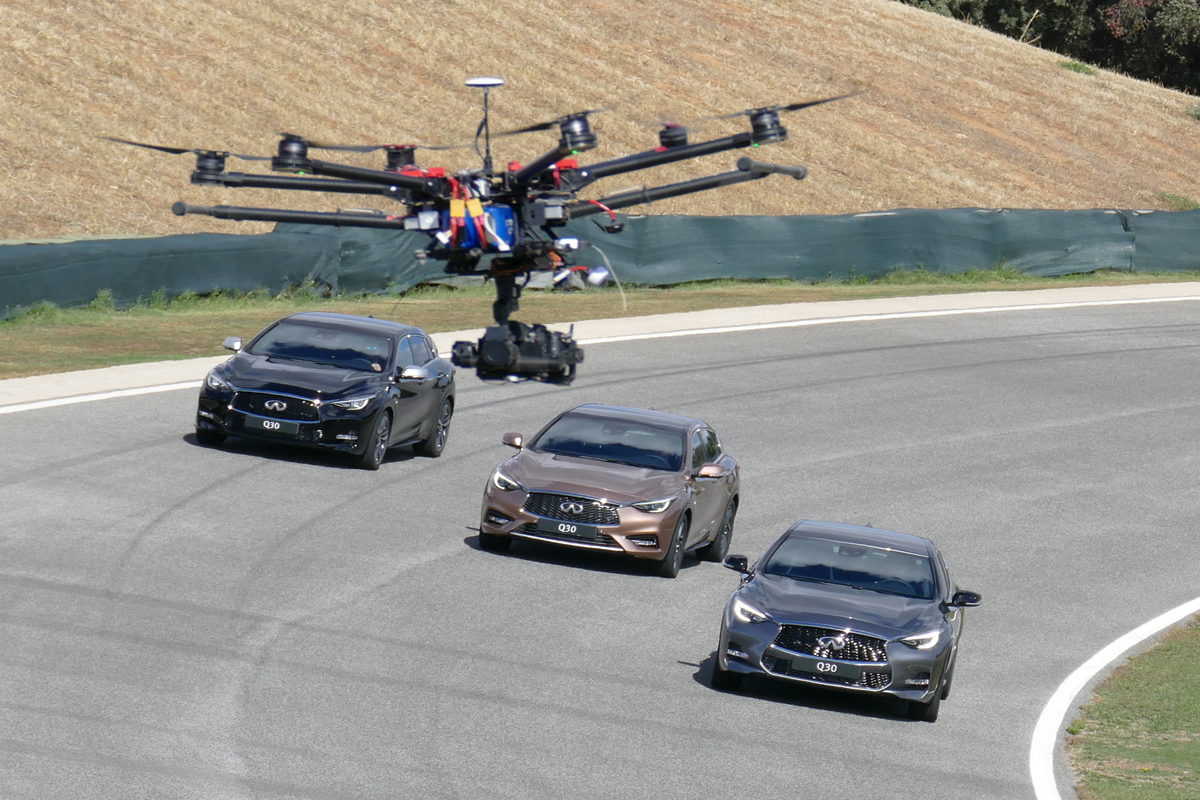
\includegraphics[width=0.4\textwidth]{imgs/anuncio_television.jpg}
				\caption{Drone grabando para la publicidad de una marca de coches.}
	\label{fig:Drone grabando publicidad.}
\end{figure}

%\subsection{Drones para el control.}
%\hspace{1 cm} En este \'area podemos destacar varios usos distintos, pero su expansi\'on en esto se debe a que con un drone podemos controlar una zona para la que anteriormente necesit\'abamos varias c\'amaras, y aun as\'i pod\'ian quedar zonas sin vigilar. \'Esta tecnolog\'ia nos lleva a poder mover una c\'amara por un lugar amplio sin necesidad de estar all\'i ni de tener un gran despliegue de elementos, as\'i como evitar que queden puntos muertos. Algunos ejemplos de esto son los siguientes: 

%\begin{itemize}
	\subsection{Seguridad} Teniendo un drone en un lugar como pueda ser una nave industrial, podemos hacer que este se desplace grabando en todo momento lo que ve, y si se detecta algo sospechoso en alg\'un lugar el drone se diriga all\'i en el momento para obtener im\'agenes de lo que est\'a pasando. 

\begin{figure}[H]
	\centering
		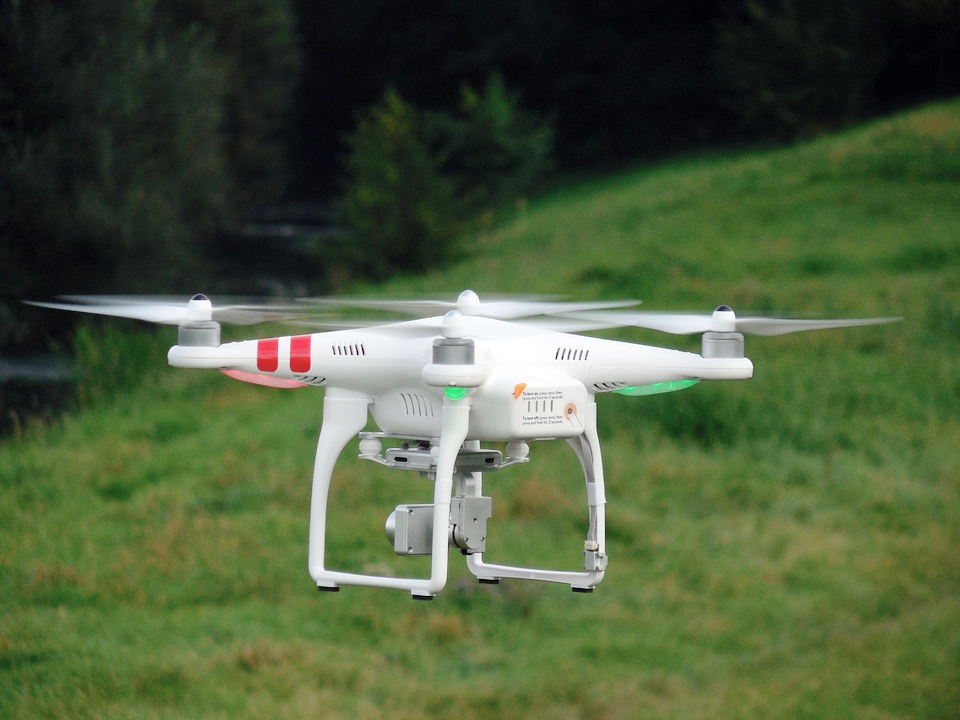
\includegraphics[width=0.4\textwidth]{imgs/seguridad_drone.jpg}
		\caption{Empresa Prevent Security Sistems utiliza drones para videovigilancia en grandes superficies .}
	\label{fig: Empresa Prevent Security Sistems realiza videovigilancia con drones.}
\end{figure}

	\subsection{Sector agr\'icola} El uso de drones en este sector se encuadra en la agricultura de precisi\'on. Se debe a la facilidad con la que un drone puede sobrevolar una zona y ofrecer im\'agenes de alta calidad, obteniendo un buen control de los cultivos en menos tiempo, con menos gasto y al tratarse de un veh\'iculo el\'ectrico al evitar desplazamientos de otros autom\'oviles conlleva un menor impacto ambiental. Adem\'as, este permite ver con facilidad el estado de la cosecha, detectar enfermedades o plagas, permiten fumigar desde el aire con mayor precisi\'on, ya que les puedes programar una ruta y que sigan \'esta. Tambi\'en podr\'ian obtener otros datos como las zonas con mas y menos agua, y obtener las condiciones del terreno y ver si son \'optimas para esperar cierto resultado. En este tipo de drones, aparte de la c\'amara son de importanc\'ia otros sensores, como los de temperatura y humedad, o infrarrojos para captar el espectro infrarrojo de las plantas. 
	
	
\begin{figure}[H]
	\centering
		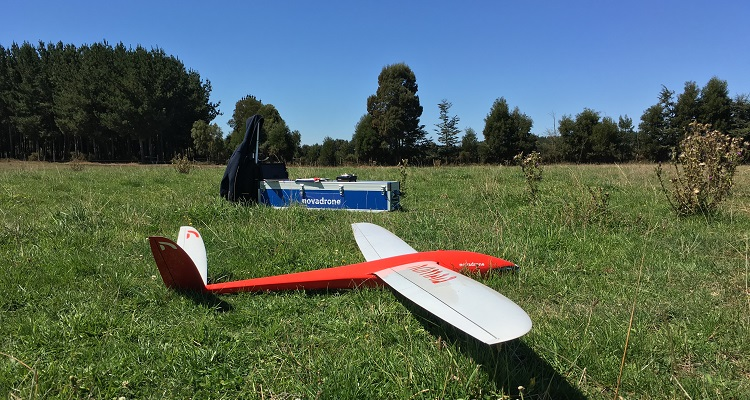
\includegraphics[width=0.4\textwidth]{imgs/novadrone.jpg}
		\caption{Empresa Novadrone utiliza drones para la gesti\'on de las explotaciones agr\'icolas .}
	\label{fig: Empresa Novadrone, aplicaciones en agricultura.}
\end{figure}

	\subsection{Inspecci\'on} En este apartado podemos englobar diversas actividades, como puede ser mantenimiento de edificios y construcciones, redes el\'ectricas o diversas instalaciones industriales como aerogeneradores e\'olicos y estados de paneles solares. Al igual que en el apartado anterior, aqu\'i podemos recorrer grandes distancias, por ejemplo para comprobar las redes el\'ectricas, sin la necesidad de que un operario pierda mucho tiempo recorriendo dicha l\'inea. Con las instalaciones solares por ejemplo, desde un plano superior podr\'iamos observar si todas las placas estan en las condiciones \'optimas y en caso de existir alg\'un fallo poder identificarlo con facilidad. Para edificios y aerogeneradores lo que hay que tener en cuenta es la altura que pueden tener, y a la cual con un drone llegar\'iamos con facilidad y observar\'iamos si hay alg\'un problema. En estos casos lo que evitamos, como anteriormente he comentado, es que alguien tenga que ir sitio a sitio perdiendo mucho tiempo. Destacando tambi\'en que este tipo de actividades se pueden implementar programas que directamente detecten las anomal\'ias, sin necesidad de que haya una persona revisando en todo momento las im\'agenes, donde tambi\'en con una inversi\'on inicial, al final ahorrar\'iamos mucho tiempo y dinero. Un ejemplo de \'esto lo podemos ver en la empresa Iberdrola, la cual ha incorporado drones para el mantenimiento e inspecci\'on de infraestructuras, utilizando drones por ejemplo para el mantenimiento de las palas de los aerogeneradores. Uni\'on Fenosa tambi\'en ha incorporado los drones para la inspecci\'on de los tendidos el\'ectricos. 
%\end{itemize}

%\hspace{1 cm} Por otro lado, pueden aportar gran ayuda en situaciones que no se dan de forma peri\'odica, sino que ocurren de forma espor\'adica y en lugares muy distintos. Gracias a los drones podemos tener una camara que nos muestre una imagen de esta zona o que nos permita ayudar all\'i, y en otro momento llevarlo a otro lado, lo que lleva a no tener un gran despliegue de medios en un lugar que apenas va a ser necesario. Los ejemplos podr\'ian ser los siguentes:

%\begin{itemize}
	\subsection{Emergencias} Cuando ocurren ciertas catastrofes naturales por ejemplo, son de gran ayuda debido a la velocidad con la que pueden llevar materiales (m\'edicos o de otro tipo) a la zona afectada. Un ejemplo de esto es el \textit{Angel Drone}, proyecto desarrollado por la universidad de S\'idney, que puede llevar materiales quir\'urgicos o plasma sangu\'ineo, por ejemplo.

\begin{figure}[H]
	\centering
		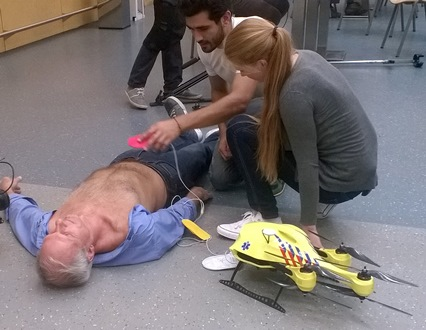
\includegraphics[width=0.4\textwidth]{imgs/drone_desfibrilador.jpg}
		\caption{Desarrollan en la universidad de Holanda un dron que lleva incorporado un desfibrilador .}
	\label{fig: Drone con desfibrilador para emergencias.}
\end{figure} 
	%\item \textbf{B\'usqueda de personas:} Al tratarse de medios que pueden sobrevolar zonas obteniendo grandes im\'agenes, pueden ser de ayuda cuando monta?eros o caminantes tienen accidentes en bosques o monta?as, quedan incomunicados y se comienza una b\'usqueda.

	%\item \textbf{Incendios forestales:} Los drones pueden estar sobrevolando zonas y obteniendo informaci\'on de esta, para as\'i poder prevenir posibles incendios o alertar lo antes posible en cuanto uno ocurra. 

%\end{itemize}

\subsection{Proyectos de empresas }
\hspace{1 cm} Es muy importante este \'ambito, pues determinados grupos y grandes empresas est\'an trabajando en su desarrollo debido al futuro que se viene por delante. Esto se debe a la facilidad que puede llevar esto para realizar grandes tareas, como el control de material en almacenes o transporte de material de un lugar a otro. Una c\'aracteristica importante es la rapidez con la que pueden llegar los drones de un lugar a otro, y acceder a lugares que es dif\'icil por otros veh\'iculos. De momento las distintas empresas que est\'an integrando esta tecnolog\'ia en el uso diario, no tienen todav\'ia proyectos terminados que realicen todas las tareas, pero si tienen distintos prototipos o proyectos piloto, de los que se pueden destacar algunos casos.


\hspace{1 cm} Por un lado, como pionero en este area se encuentra \textbf{Amazon}, el cual lleva desarrollando desde 2013 una tecnolog\'ia que permita el reparto de paquetes mediante drones. La idea cuenta con doce prototipos, debido en parte a los distintos tipos de UAV que tienen.  Esta tecnolog\'ia lleva consigo los llamados almacenes a\'ereos, es decir, un almac\'en que se mantendr\'ia en el aire gracias a dirigibles, el cual tiene paquetes a entregar y drones. El drone obtendr\'ia el paquete que se debe entregar y lo llevar\'ia al lugar adecuado. Tras esto volver\'ia a un almacen hasta que se le mande de nuevo al almac\'en a\'ereo para el siguiente reparto. Estos drones sabr\'ian en todo momento en el estado y en el punto en el que se encuentran, es decir, que saben a qu\'e lugar deben ir dependiendo de la tarea a realizar. 

\begin{figure}[ht]
	\centering
		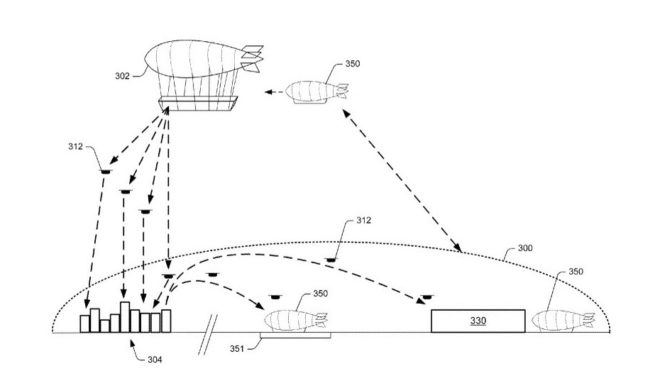
\includegraphics[width=0.55\textwidth]{imgs/amazon.jpg}
	\label{fig:Esquema de reparto con drones}
\end{figure}

\hspace{1 cm} Por otro lado, tambi\'en para el reparto de mercancias se encuentra \textbf{Google}, llegando a tener un programa piloto en Australia en el año 2014, pero no consigui\'o llevarlo a Estados Unidos. Aun as\'i, consigui\'o hacer pruebas en una universidad de reparto de comida, un reto que supuso principalmente que la comida llegara r\'apido a su destino y en buenas condiciones. Adem\'as tambi\'en sirvi\'o para ajustar los sistemas autom\'aticos de vuelo y entrega de la mercancia. 

\hspace{1 cm} A ra\'iz de estos servicios de entregas, se ha producido otro desarrollo importante, como puede ser el de tener controlados los paquetes dentro de un almac\'en. Un pionero de esto ha sido un grupo en el \textbf{MIT}, desarrollando un sistema que permite a los drones moverse por los almacenes escaneando los c\'odigos de cada paquete, enviando esta informaci\'on a un servidor y que este pueda tener controlados los paquetes que hay y donde est\'an situados. 

\begin{figure}[H]
 \centering
  \subfloat[RFID detectado]{
   \label{f:RFID detectado}
    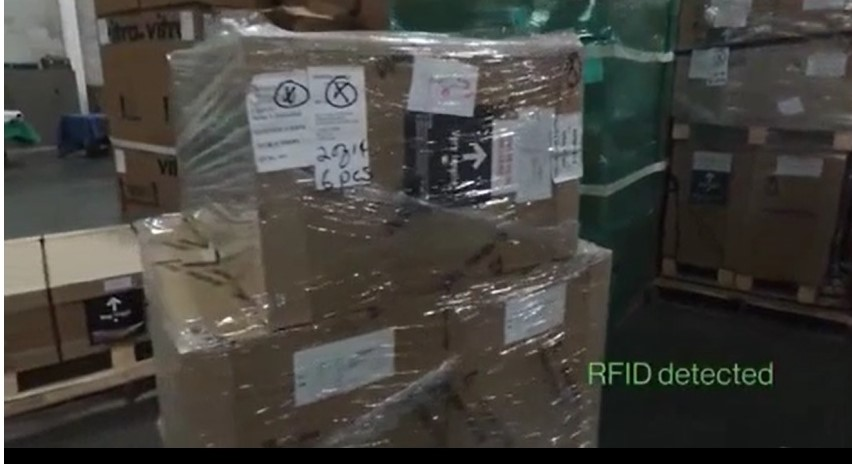
\includegraphics[width=0.33\textwidth]{imgs/MIT1.jpg}}
  \subfloat[RFID decodificado]{
   \label{f:RFID decodificado}
    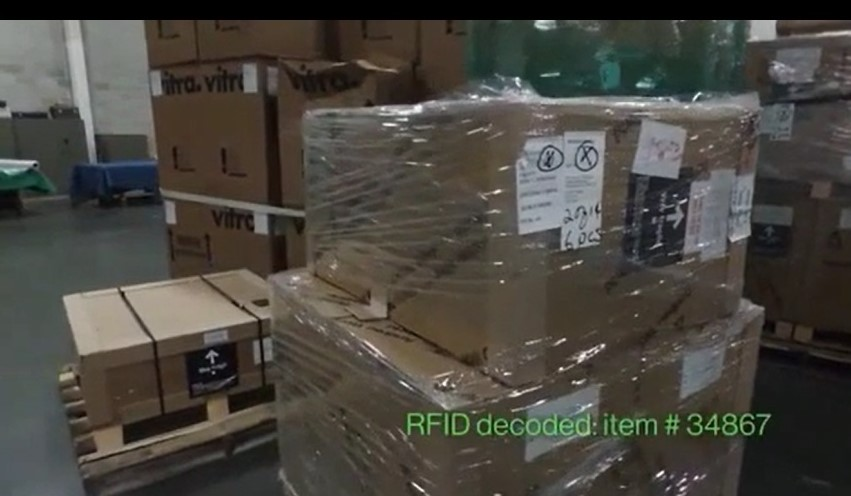
\includegraphics[width=0.33\textwidth]{imgs/MIT2.jpg}} 
  \subfloat[Item RFID localizado]{
   \newline\label{f:Item RFID localizado}
    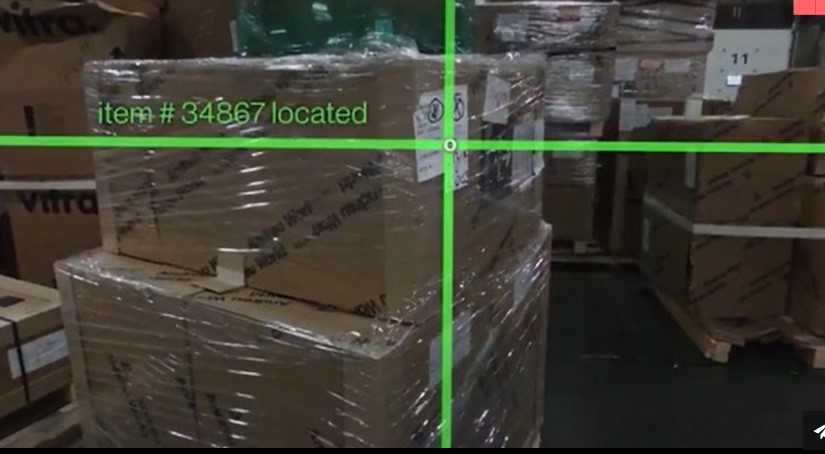
\includegraphics[width=0.33\textwidth]{imgs/MIT3.jpg}} 
 \caption{Drone detectando codigo RFID.}
 \label{f:Drone detecta codigo RFID}
\end{figure} 


\hspace{1 cm} Para el traslado de mercancias en interiores tambi\'en se ha puesto en marcha la cadena de supermercados estadounidense Walmart, cuyo objetivo es transportar productos de un lugar a otro previamente establecidos. La idea de este proyecto se debe a los grandes almacenes que tienen estos supermercados, y que cuando un cliente no encuentra el producto deseado, avisa a un empleado y \'este tiene que ir al almacen a buscarlo, perdiendo mucho tiempo entre la distancia recorrida y la b\'usqueda del producto. Lo que conseguir\'ian con esto, es que en caso de que los empleados est\'en ocupados, un cliente no tenga que estar a la espera, sino que con un dispositivo podamos pedir el producto y un drone se encargar\'a de ir a por el y traerlo al punto donde nos encontremos. Destacar que se incorporaran en las tiendas controladores a\'ereos para que los veh\'iculos sigan una trayectoria segura.  



\section{Hardware}
\hspace{1 cm} Hay que destacar las partes que tiene un drone y su forma, pues es gran parte lo que lo hace tan especial, permite que tenga una gran libertad de movimientos, ya que puede moverse sin problema desde cualquier punto hacia los ejes X, Y y Z. Lo que ganamos con esto son cosas como poder permitirse un aterrizaje y un despegue totalmente vertical, sin depender de un espacio en el que coger velocidad para poder levantar el vuelo, e igual con el aterrizaje, pudiendo el drone estando quieto en el aire bajar totalmente en vertical hasta tocar posarse sobre el suelo. Una vez en el aire pueden moverse adelante, atr\'as, izquierda, derecha, arriba, abajo y combinaciones de movimientos entre ejes, adem\'as de los movimientos Roll, Yaw y Pitch y sin necesidad de hacer movimientos bruscos. Sin embargo, en los anteriores UAV solo tenemos el movimiento hacia adelante, teniendo que jugar con Roll, Yaw y Pitch para poder movernos en los distintos ejes.

\begin{figure}[ht]
	\centering
		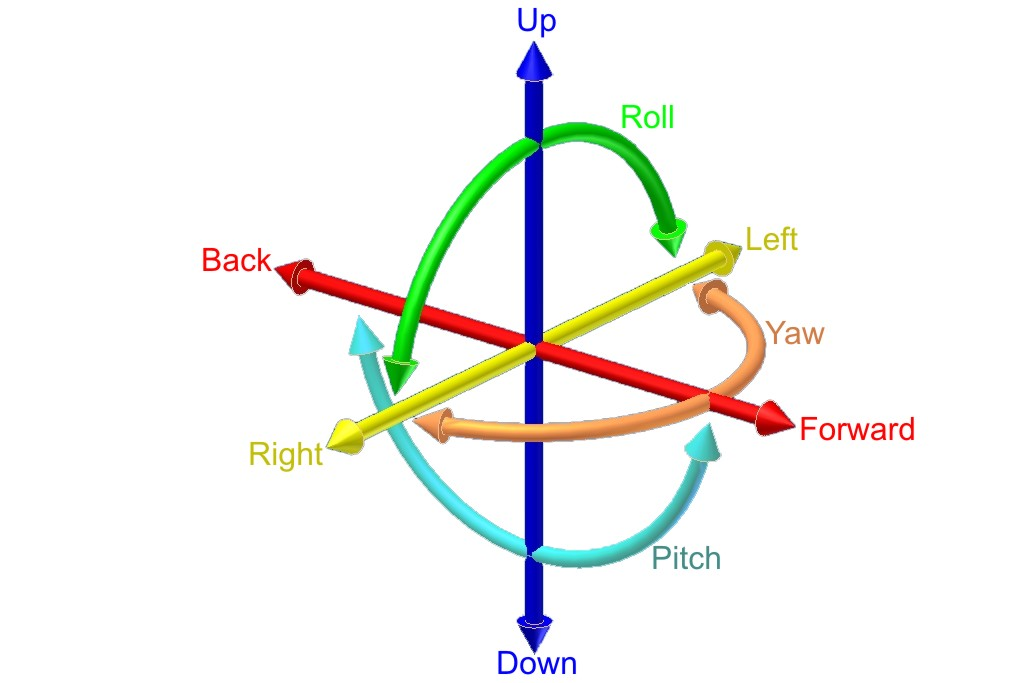
\includegraphics[width=0.3\textwidth]{imgs/ejesdrone.eps}
		\caption{Esta imagen muestra los movimientos que tiene un dron.}
	\label{fig:ejesdrone}
\end{figure}

\hspace{1 cm} Explicado esto, un desglose explicando cada una de las partes ser\'ia :

\hspace{1 cm}\textbf{Frame:} Tambi\'en conocido como marco, estructura o chasis. Es la estructura principal sobre la que se sit\'uan el resto de los elementos. Cambiar\'a su forma dependiendo del drone, variando la longitud de las patas o el n\'umero de soportes para h\'elices, por ejemplo. Esta puede estar hecha por diversos materiales, generalmente se trata de alg\'un tipo de pl\'astico, ya que es un material que tiene poco coste y pesa poco. Un ejemplo es el polipropileno, que es ligero y con mucha resistencia, lo que permite colocar sobre el la bater\'ia. Otro material que suele utilizarse es la fibra de carbono, ya que se trata de un material que pesa poco y es muy resistente, aunque puede tener factores negativos como su conductividad. Por ultimo, tambi\'en nombrar la fibra de v\'idrio. Este material tambi\'en es muy utilizado por ser ligero, y tiene caracter\'isticas como que no es conductor de la electricidad. Es com\'un ver estructuras h\'ibridas entre distintos materiales, sobre todo juntando los dos tipos de fibra. 

\hspace{1 cm}\textbf{H\'elices:} Elemento formado por dos palas montadas de forma conc\'entrica sobre un eje, que al girar crean un par de fuerzas, permitiendo as\'i el movimiento del dron.

\hspace{1 cm}\textbf{Motores:} Son los encargados de transformar la energ\'ia que llega en movimiento sobre el eje en el que se sit\'uan las h\'elices, para as\'i permitirles a \'estas hacer su trabajo. Este, a su vez, tiene distintos par\'ametros que ser\'an principalmente los que permitan al drone llevar mayor velocidad. 

\hspace{1 cm} El numero de vueltas que d\'e por minuto, lo que depender\'a de los KiloVoltios. Suele estar en torno a 800-900kV.

\hspace{1 cm} El tamaño que \'este tenga. Al mirar las especificaciones de un drone est\'a en un numero de 4 d\'igitos, en el que los dos primeros hacen referencia al tamaño del rotor y los otros dos al tamaño de la bobina. 

\hspace{1 cm} El empuje, valor que hacer referencia al peso que puede levantar el motor.

\hspace{1 cm} La corriente, se trata de la energ\'ia (amperios) que se consume cuando el motor est\'a al m\'aximo.


\hspace{1 cm}\textbf{Bater\'ia:} Encargada de proporcionar la energ\'ia suficiente para que el drone pueda realizar un vuelo, permitiendo trabajar a la placa controladora y motores. La caracter\'istica principal de las bater\'ias son los miliamperios, ya que es la que permitir\'a una mayor capacidad y por lo tanto que el drone tenga un mayor tiempo de vuelo. Existen bater\'ias de muy diversos tamaños, desde los 350 mah en drones de juguete a, por ejemplo, los 4500mah que tiene la bater\'ia del drone 3DR solo. Tambi\'en es importante la tasa de descarga, que se trata de la m\'axima energ\'ia que puede entregar y el periodo de tiempo durante el que puede hacerlo. Normalmente los drones traen sistemas de alerta que avisan cuando a la bater\'ia le queda poca energ\'ia, o que cuando queda un valor menor a cierto porcentaje de carga no permite despegar el drone, evitando as\'i que se quede sin energ\'ia a mitad de un vuelo.

\hspace{1 cm}\textbf{Equipo de transmisi\'on:} Es el encargado de que se comunique el drone con una estaci\'on receptora. Puede variar en funci\'on del aparato ya que se pueden usar diferentes tecnolog\'ias, pero principalmente se trata de radiofrecuencia o de Wifi. Existen casos, como el modelo 3DR, que combina ambas tecnolog\'ias, utilizando la radiofrecuencia para la informaci\'on del movimiento, bater\'ia y posicionamiento, y el WiFi para la transmisi\'on de im\'agenes en directo. Podemos encontrar distintos equipos de sistemas de transmisi\'on, uno de los \'ultimos y mas destacables es \textbf{Hyperion}, que utiliza un sistema \'optico de comunicaciones capaz de transmitir hasta 1Gb por segundo, lo que permite la transmisi\'on de datos mediante la luz directa. La principal caracter\'istica de \'este es que no pierde informaci\'on cuando no hay contacto directo entre las dos estaciones. Pero v\'ia WiFi es algo muy utilizado en los \'ultimos momentos, pues permite controlar el dron desde una aplicaci\'on movil, por lo que conectando estos dos tendr\'iamos un mando que nos permite cambiar gran parte de la configuraci\'on del drone. Tambi\'en existen dispositivos que permiten el control mediante Bluetooth, pero \'este es menos com\'un ya que tiene mayor restricci\'on de velocidad de datos y distancia. 


\hspace{1 cm}\textbf{Placa controladora:} Es el procesador del drone, el que se encarga de recoger la informaci\'on del drone y cuando le llega una orden ver que informaci\'on tiene que mandar para que \'esta se ejecute de forma correcta, as\'i como en caso de haber un problema tratar de evitarlo. Es b\'asicamente el hardware que utiliza el drone. Hay una gama muy amplia dentro de \'este,donde cabe destacar \textbf{Pixhawk}, pero podemos encontrar varias con gran trascendencia: 
	\begin{itemize}
		\item Pixhawk: Es el m\'as utilizado debido a que trabaja con 3DRobotics y Ardupilot. Sirve para diversos dispositivos como son drones, helic\'opteros y barcos. Est\'a pensado para cualquier veh\'iculo que tenga movimiento. Se trata de un proyecto hardware abierto, cuyo objetivo principal es proporcionar el hardware de autopiloto a comunidades acad\'emicas o gente que tiene esto como un hobby, teniendo as\'i un bajo costo y una alta disponibilidad. Se trata de un piloto autom\'atico en tiempo real y muy eficiente, proporcionando un entorno de estilo POSIX. \'Este es el autopiloto est\'andar de la industria, y por lo tanto, como veremos a continuaci\'on, a partir del cual se han desarrollado diversos autopilotos con distintas mejoras. 

		\item Pixhawk2: Es una versi\'on avanzada de la placa anterior. Tiene mejoras como aislamiento de vibraciones, 3 IMUs para redundancia (3 aceler\'aometros, 3 giroscopios, 3 magnet\'ometros y 2 bar\'ometros) y sensor para controlar la temperatura. 

		\item PixRacer: \'Este se ha desarrollado para los drones de carreras, aunque tambi\'en se utiliza en minidrones. Suele tener una mayor memoria flash.

		\item Navio2: Piloto autom\'atico diseñado de Raspberry Pi. Te permite convertir esta en un controlador de drone. 

		\item PXFmini: Se trata de otro piloto autom\'atico de Raspberry Pi. \'Este tiene la electr\'onica para la mayor\'ia de los componentes que puede utilizar un dron. 

		\item FlytPOD: Se trata de una placa Odroid XU4 SBC junto con una PixHawk. Puede volar diversos veh\'iculos a\'ereos y su principal caracter\'istica es el WiFi que tiene integrado. Existe una placa FlytPOD pro que se trata de una versi\'on extendida de la anterior, teniendo todas sus caracter\'isticas, pero con m\'as sensores y mayor capacidad de almacenamiento. 

		\item U-Pilot: Este hardware se caracteriza por servir para diversos vehi\'iculos a\'ereos, siendo programable para realizar todas las acciones de su camino de forma autom\'atica. Su radioenlace con frecuencia en torno a 900Mhz permite controlar el dispositivo a una distancia de 100km. 
	\end{itemize}

\hspace{1 cm} Hay que destacar un elemento importante como es la \textbf{c\'amara}, que aunque no todos los drones la llevan s\'i que es algo bastante com\'un. Algunos la llevan incorporada (incluso dos c\'amaras, una que apunta hacia la parte de delante y otra que apunta la parte de abajo) y otras que traen soporte para poder incorporar ciertas c\'amaras, normalmente consideradas camaras de acci\'on, para as\'i obtener una mejor calidad, e incluso incorporar adaptadores como puede ser una Gimbal para controlar la parte hacia la que queremos que apunte la c\'amara en cada momento o utilizarlo como estabilizador, para evitar as\'i que afecten a la imagen diversos movimientos, generalmente bruscos, que pueda realizar el drone. Cabe destacar que en muchas ocasiones, utilizado normalmente para carreras de drones, la c\'amara sirve para integrar la tecnolog\'ia FPV (First Person View), que es junto a la c\'amara, el transmisor de v\'ideo y el receptor de v\'ideo, poder ver en tiempo real las im\'agenes sobre una pantalla LCD o utilizando unas gafas de realidad virtual. En este aspecto, en los \'ultimos años se ha visto por otro lado un gran avance de la realidad virtual, y es tambi\'ien hay una gran variedad en este mundo, pues existe una gama que va desde las \emph{cardboard}, que permiten con un trozo de cart\'on y un par de lentes, poniendolos de cierta forma y con el uso de un smartphone, tener de forma sencilla unas gafas 3D, hasta gafas para la videoconsola que te permiten entrar en el videojuego, añadiendo una gran calidad de imagen y con un sonido envolvente para entrar de lleno en el ambiente. Pero una de las cosas mas impactantes es el conjunto que se ha creado con el done \textbf{FLYBi}, estando \'este conectado a unas gafas de realidad virtual que tienen sensor de movimiento, lo que te permite sentir que eres t\'u el que vuelas y el que est\'as en el lugar del dron, y con cualquier movimiento que sientan las gafas la c\'amara del drone lo imitar\'a. En caso de que esto parezca inc\'omodo el drone tiene un joystick con el que enviar\'a la informaci\'on de los elementos a realizar a la c\'amara. 
 

\begin{figure}[H]
 \centering
  \subfloat[Chasis]{
   \label{f:chasis}
    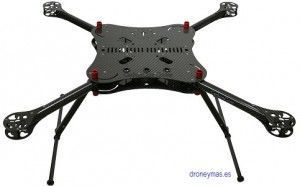
\includegraphics[width=0.2\textwidth]{imgs/chasis-drone.jpg}}
  \subfloat[Helices]{
   \label{f:helices}
    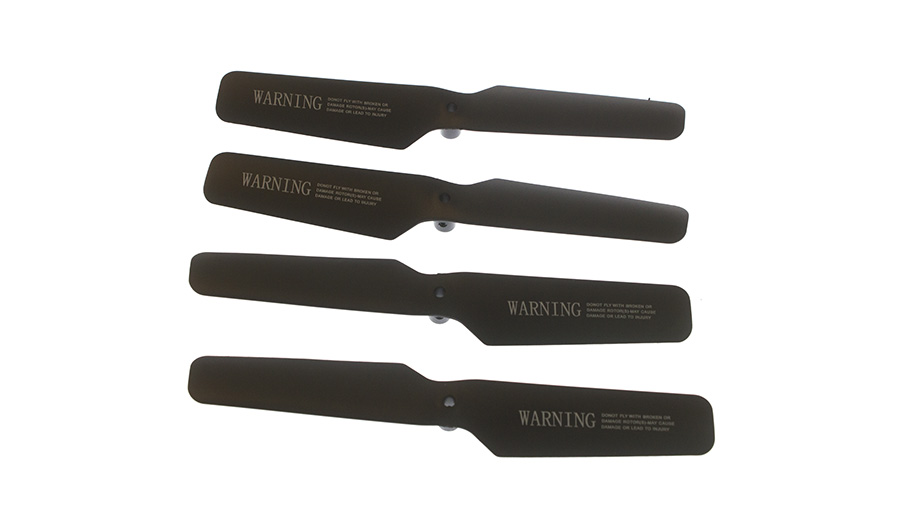
\includegraphics[width=0.2\textwidth]{imgs/helices-drone.jpg}}
  \subfloat[Motor]{
   \newline\label{f:motor}
    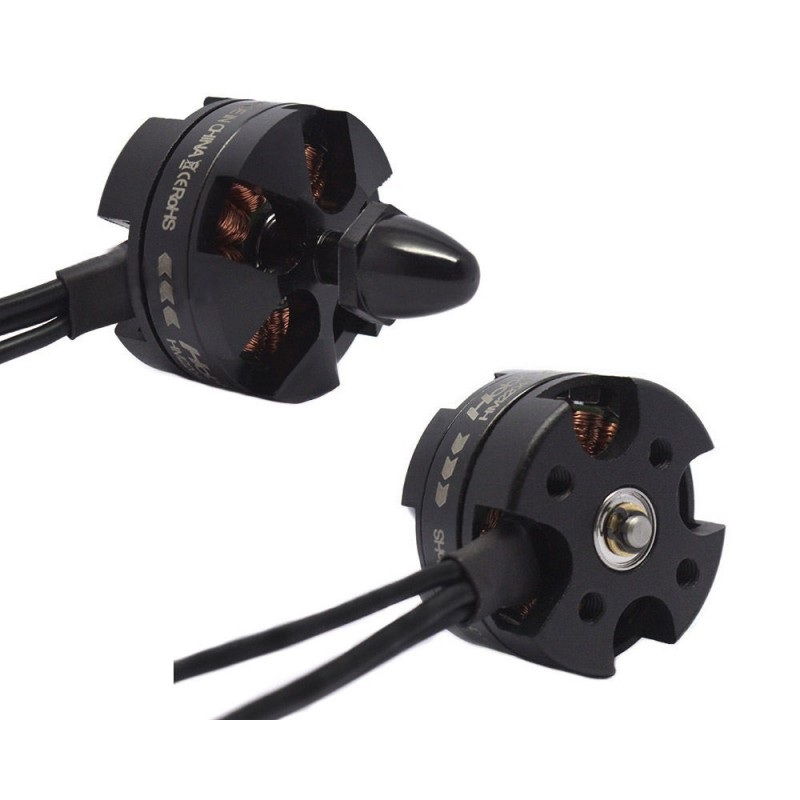
\includegraphics[width=0.2\textwidth]{imgs/motor-drone.jpg}}
	\subfloat[Placa-Madre]{
   \newline\label{f:placa-madre}
    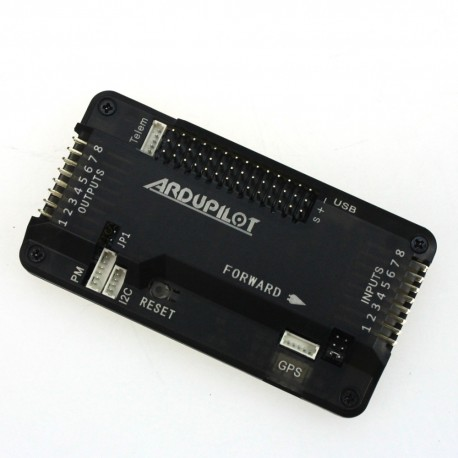
\includegraphics[width=0.2\textwidth]{imgs/placaControladora-drone.jpg}}
 \caption{Distintas partes del drone.}
 \label{f:Test 1}
\end{figure} 


\section{Software}
\hspace{1 cm} Como sabemos, el software es el conjunto de programas que van a permitir realizar ciertas tareas, en este ser\'a lo que permita realizar al drone una navegaci\'on aut\'onoma. Dicho programa estar\'a instalado en la placa controladora, y por tanto sera el que ejecute para recoger la distinta informaci\'on de los sensores, procesar la informaci\'on y enviar las \'ordenes correctas a los distintos elementos de \'este. Como se ha comentado anteriormente, el desarrollo de software para este tipo de robots ha evolucionado mucho en los ultimos años debido al uso civil que se le comienzan a dar y no tanto al desarrollo militar. Es importante destacar el software de \textbf{ArduPilot}, ya que se trata del software auto-piloto m\'as avanzado, pero existen tambi\'en otros que nos permiten el manejo de estos robots:

	\begin{itemize}
		\item \textbf{Ardupilot:} Es un sistema OpenSource encargado de recibir la informaci\'on que se le da y de esta forma enviar las señales correspondientes a los actuadores. Se trata del software m\'as importante debido a lo completo que es y confiabilidad que proporciona, debido a la gran cantidad de gente que lo utiliza (pilotos de drones profesionales y aficionados) y por el equipo de ingenieros que lo han desarrollado. Este software se caracteriza por la variedad de dispostivos que puede llegar a controlar, ya que trabaja con diversos dispositivos a\'ereos (aviones, helic\'opteros, drones, etc) y con dispositivos marinos (como pueden ser los barcos y submarinos). \'Este ha tenido un gran desarollo debido a su principal caracter\'istica: Opensource. Hay mucha gente creando interfaces para este y dichos usuarios comparten sus avances con el resto. A partir de \'este han nacido controladores como Ardupilot Mega. El problema que tiene dicho software es que s\'olo permite trabajar con plataformas de los mismos creadores, lo que lleva al siguiente software. Otra caracter\'istia es la facilidad con la que se le pueden añadir diferentes sensores, como pueden ser modulos GPS o c\'amaras, algo que facilitar\'a la navegaci\'on aut\'onoma. 

	\item \textbf{Megapirate-NG:} Apareci\'o como desarrollo del anterior. La funcionalidad de uno y otro es practicamente la misma, con la diferencia de que \'este permite trabajar con Hardware de otros creadores. El problema es que siempre depende de Ardupilot, por lo tanto sus funcionalidades, aunque sean mas c\'omodas para trabajar, puede que esten atrasadas.

		\item \textbf{MultiWii:} \'Este se propuso como radiocontrol para drones. Es un sistema que fue creado por los desarrolladores y con los sensores (giroscopios y aceler\'ometros) de la Nintendo Wii. Es una plataforma basada en arduino, con el factor en contra de tener una funcionalidad bastante limitada. 
	\end{itemize}


Estos primeros son los softwares principales que estar\'ian sobre el veh\'iculo, pero tambi\'en estan los programas que se ejecutar\'ian en otros dispositivos como el ordenador o el tel\'efono m\'ovil para ver la informaci\'on que este nos env\'ia. Normalmente el fabricante del drone tiene ya un programa que realiza esta funci\'on. 

\hspace{1 cm} En este punto es importante el protocolo de comunicaci\'on que habr\'a para comunicarse el veh\'iculo con la estaci\'on terrena. Aqu\'i hay un protocolo que destaca sobre los dem\'as, el \textbf{MAVLink} (Micro Air Vehicle Communication Protocol). \'Este protocolo tiene la informaci\'on contenida en ficheros .xml, lo que permite utilizarlo en diversos lenguajes de comunicaci\'on, lo que conlleva una mejora notable en su desarrollo. Al tener el fichero .xml los tipos de mensaje, permite con facilidad a?adir nuevos tipos para asignar una tarea nueva a cada uno. Otra ventaja de este es que hay muchos software de drones que lo soportan, como pueden ser Ardupilot, Autopilot, algunos derivados de estos y otros como Gentlenav o Flexipilot, y desde la estaci\'on tierra algunos como MAVProxy, Mission Planer o APM planner. 
Un problema en este protocolo es que los datos no estan encriptados en la comunicaci\'on, por lo que es mas facil un ataque y que se manipulen los datos, siendo detectable si se hace perder algun dato ya que se utiliza CRC (codigo de redundancia c\'iclica para detectar cambios en los datos, este se utiliza en protocolos como TCP).
MAVLink utiliza otro software llamado MAVProxy para poder acceder a los datos del veh\'iculo, como la velocidad y las im\'agenes, lo que nos permitir\'a tambi\'en saber que datos mandarle para que funcione de forma correcta. 

\hspace{1 cm} A parte de todos estos, existen tambi\'en otras infraestructuras software como puede ser \textbf{JdeRobot}. En s\'i JdeRobot se trata de un software de desarrollo para rob\'otica y aplicaciones de visi\'on por computador. \'Este puede trabajar con distintos sensores que le proporcionan informaci\'on, en caso del drone con la informaci\'on que le permite Ardrone Server, y gracias a esto puede controlar el dispositivo y ver los distintos datos. Con JdeRobot es muy sencillo tomar el control del hardware gracias a su programa de control. Tiene una gran API que permite realizar diversas tareas como trabajar con aparatos reales o simulados, y conectarse a ellos de forma local o a trav\'es de la red. Decir que para el trabajo realizado, esta plataforma ha sido muy importante, pues su componente para la c\'amara, su aplicaci\'on para filtros de color y la posibilidad de realizar diagramas de estado permite tener en todo momento datos importantes del dron y poder mantenerlo bajo control sin ning\'un problema. Destacar que se trata de un sistema OpenSource que permite trabajar con simuladores como Gazebo y con ayuda de librerias como OpenCV. 
 


	

\section{Rob\'otica a\'erea en el laboratorio de la URJC}
\hspace{1 cm} Es importante destacar que el inicio de este proyecto se ha podido dar gracias a otros proyectos realizados en el laboratorio de la universidad, en los que se hicieron grandes avances en el \'area de la rob\'otica a\'erea y que nos han llevado a centrarnos en el caso de la situaci\'on por visi\'on mediante balizas. Algunos casos de otros trabajos son los siguientes:

\hspace{1 cm} Alberto Mart\'in trabaj\'o en la navegaci\'on visual para el seguimiento de objetos. En este proyecto el drone trabajaba en los ejes X,Y y Z. Teniendo un objeto de determinadas caracter\'isticas el drone era capaz de seguirlo, funcionando tanto en el eje vertical como en el horizontal. Tambi\'en era capaz de cambiar la orientaci\'on del drone en funci\'on de la situaci\'on del objeto. 

\hspace{1 cm} Daniel Yag\"ue trabaj\'o en con el ArDrone sobre gazebo, probando distintas funcionalidades y distintos escenarios. En este proyecto, tambi\'en mediante control visual, realiz\'o diversas pruebas como seguir l\'ineas, seguir otro drone o seguir un recorrido mediante April Tags. 

\hspace{1 cm} Manuel Zafra trabajo en la localizaci\'on del Drone mediante April Tags. En este proyecto el drone iba detectando las diferentes April Tags que hab\'ia situadas en los distintos lugares y gracias a ello sab\'ia la posici\'on en la que se encontraba y los movimientos a realizar.  

\hspace{1 cm}Arturo Velez realiz\'o un proyecto en el cual el drone segu\'ia un objeto dada una textura y la autolocalizaci\'on a partir de \'esta. Si no se encontraba la textura el drone realizaba una b\'usqueda. Tambi\'en trabaj\'o con April Tags y la autolocalizaci\'on en funci\'on de lo que detectaba.

\hspace{1 cm} Por \'ultimo nombrar el proyecto de Jorge Cano, quiz\'as es el mas distinto a los anteriores y a lo que se ha trabajado aqu\'i, ya que se centraba m\'as en el hardware del drone, especificando los distintos materiales y su configuraci\'on con el software. Destacar que tami\'en realiz\'o pruebas de vuelo para las cuales tuvo que trabajar en las partes perceptiva y de control.

\hspace{1 cm} Una vez terminada la breve introducci\'on, se va a explicar lo realizado en este proyecto. El orden seguido ha sido el siguiente:

\hspace{1 cm} En el cap\'itulo 2 se redactan los objetivos propuestos y la metodolog\'ia seguida para llegar hasta ellos. 

\hspace{1 cm} En el cap\'itulo 3 se redacta la infraestructura utilizada y como se ha trabajado con ella. 

\hspace{1 cm} En el cap\'itulo 4 se redacta el algoritmo realizado, como se ha programado y porque se han seguido unos u otros caminos.

\hspace{1 cm} En el cap\'itulo 5 se redacta los distintos experimentos realizados y los resultados que se han obtenido.

\hspace{1 cm} Por ultimo, en el cap\'itulo 6 se redactan las conclusiones a las que se han llegado tras finalizar este proyecto.


\lhead[]{CAPÍTULO \thechapter. OBJETIVOS}
\chapter{Objetivos}\label{cap.Objetivos}
En este capitulo se van a explicar los objetivos a conseguir y el metodo utilizado para llegar a ello.

\section{Objetivo principal}
\hspace{1 cm} El objetivo propuesto para este trabajo era conseguir que un drone navegara de forma aut\'onoma. Para ello la idea era situar el drone en un punto de inicio, despegara sobre este y una vez se hubiera estabilizado comenzara a desplazarse siguiendo un algoritmo de b\'usqueda previamente programado. La idea de este es recorrer determinado area sin la necesidad de pilotar el drone. Los movimientos de este drone dependerian de lo que detectara la c\'amara en cada momento. Esta b\'usqueda se realizar\'ia con la finalidad de encontrar una baliza sobre la cual aterrizar. En caso de no ver la baliza, el drone se moveria realizando una espiral en busqueda de esta, en el caso de encontrarla el drone se situar\'ia sobre esta y una vez centrado aterrizar\'ia. Esta baliza seria un cuadrado formado por cuatro cuadrados de colores distintos. 

\begin{figure}[H]
	\centering
		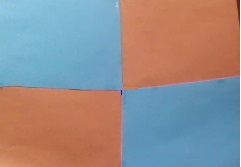
\includegraphics{imgs/baliza.jpg}
	\label{fig:Baliza elegida sobre la que aterrizar. }
\end{figure}

\hspace{1 cm} Para conseguir este objetivo, hay que tener en cuenta varias partes importantes, de las cuales a partir de una pasamos a la otra para al final llegar a lo que permitir\'a el correcto funcionamiento del algoritmo: que los movimientos de este dependan de lo que ve la c\'amara.

\begin{itemize}
	\item \textbf{Creaci\'on de un filtro de color:} Gracias a los colores podemos detectar los cuadrados de la baliza, por lo que realizando este filtro obtendremos estos objetos y los que sean del mismo color, eliminando as\'i informaci\'on no necesaria de la imagen.
	
	\item \textbf{Detecci\'on de objetos: } Tras el filtro de color y eliminada informaci\'on no necesaria, podemos obtener distintos objetos en la imagen, viendo si cumplen caracter\'isticas como tener un determinado area, para as\'i saber si son los objetos que se desean o no y trabajar con ellos o descartarlos. 
	
	\item \textbf{Movimiento del drone: } Una vez obtenemos informaci\'on de la imagen y la hemos procesado, en funci\'on de esto se pretender\'a que el desplazamiento del drone sea uno u otro, trabajando asi de forma fluida y sin movimientos bruscos que puedan desestabilizarlo.   

\end{itemize}


\section{Metodolog\'ia}
\hspace{1 cm} Para poder conseguir todo esto, era necesario saber las plataformas con las que ser\'ia posible, donde tiene gran importancia el software JdeRobot, pues gracias a su desarrollo que permite la comunicaci\'on con el dron, y de estas forma obtener los datos de sus sensores, principalmente de la camara. Para este apartado fue primordial el aprendizaje de sus distintas herramientas, hubo que hacer pruebas con estas y ver su funcionamiento tanto en entornos simulados como en reales.

\hspace{1 cm}Una vez se realizaron las primeras pruebas con robots, se propuso un desarrollo en espiral. Para este desarrollo se proponian semanalmente reuniones con el tutor, en las cuales se proponian unos objetivos a seguir en funci\'on de lo que se hab\'ia conseguido hasta el momento. Una vez propuestas estas tareas se evaluavan los distintos riesgos que se pod\'ian tomar en funci\'on de trabajar de una forma u otra, y los avances a los que se pod\'ia llegar por cada camino. Una vez hecho esto se comenzaban a desarrollar los algoritmos para conseguir estos objetivos en funci\'on de la forma elegida. Una vez se realizaban estos y se probaban (en simulaci\'on o con el robot real, dependiendo del objetivo), se propon\'ia otra reuni\'on para determinar si los avances eran los deseados o no, y en funci\'on de esto planear unos objetivos u otros.  

\begin{figure}[H]
	\centering
		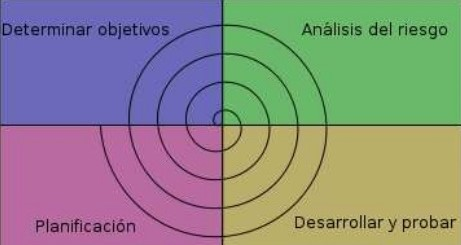
\includegraphics{imgs/metodologia-espiral.jpg}
	\label{fig:Desarrollo en espiral}
\end{figure}

\hspace{1 cm} Los avances que se iban realizando semana a semana, se subian mediante videos o imagenes a un mediawiki en JdeRobot, quedando reflejados todos los procesos. Tambi\'en se ha utilizado GitHub para subir el c\'odigo desarrollado.  

\section{Plan de trabajo}
\hspace{1 cm} El primer punto fue comprender las distintas herramientas de JdeRobot y trabajar con ellas. Creando programas simples y viendo que funcionaban, as\'i como trabajar con distintos robots reales para tener una toma de contacto con ellos y no basarse solo en un trabajo sobre simulador. 

\hspace{1 cm} En segundo lugar hubo que comprender la importancia que tendria la biblioteca OpenCV en este proyecto y ver sus multiples opciones, todo lo que permitia trabajar con imagenes y los cambios que podiamos hacer sobre estas para obtener datos deseados a partir de los cuales mandar informaci\'on. 

\hspace{1 cm} Por ultimo quedaba unir estas dos tecnolog\'ias y conseguir un buen algoritmo que nos permitiera enviar informaci\'on a tiempo real a un drone y que este la ejecutara de forma correcta y fluida.  





\lhead[]{CAPÍTULO \thechapter. INFRAESTRUCTURA}
\chapter{Infraestructura utilizada}\label{cap.infraestructura}
\hspace{1 cm} Despu\'es de fijar los objetivos concretos de este TFG, en este cap\'itulo se va a hablar sobre las distintas tecnolog\'ias utilizadas, tanto hardware como software, y el uso que han tenido en este proyecto. 

\section{Parrot AR.Drone 2.0 }
\hspace{1 cm} \'Este ha sido el drone utilizado para hacer las pruebas en un entorno real y comprobar as\'i que el desarrollo del algoritmo era el correcto. 

\hspace{1 cm} La \textsl{bater\'ia} era de 1500mah, siendo la duraci\'on en tiempo de vuelo de unos 12 minutos. %, lo que en algunas ocasiones nos ha llevado a problemas, pues el tiempo de vuelo con esto es unos 12 minutos aproxim\'adamente. Esto conllevaba que algunas pruebas en ocasiones eran muy dif\'iciles de realizar, ya que si no sal\'ia el resultado esperado en los primeros intentos, muchas veces hab\'ia que parar la prueba durante bastante rato para continuar. Si las pruebas no eran de vuelo sino que era de imagen, con este tiempo era suficiente, ya que el dron no gastaba tanta energ\'ia al relizar solo la retransmisi\'on de los datos que obten\'ia la c\'amara. Un detalle curioso en este punto es el cambio de funcionamiento que se notaba una vez la bater\'ia estaba por debajo del 30/100, pues el despegue se hac\'ia con menos fuerza y de forma m\'as inestable, adem\'as las instrucciones de movimiento que se le mandaban las ejecutaba con menos fuerza y por lo tanto de forma m\'as lenta. La \'unica soluci\'on posible para remediar este problema fue trabajar a la vez con 3 bater\'ias, pero he de decir que en momentos que las pruebas eran muy continuas durante mucho tiempo, llegaba un momento que hab\'ia que parar porque el tiempo de carga no era suficientemente r\'apido comparado con el de las 3 descargas. 

\hspace{1 cm} El \textsl{alcance} que tiene \'este con la estaci\'on tierra es de 50 metros, suficiente para las pruebas que han sido realizadas en este proyecto. 

\hspace{1 cm} Este drone tiene una \textsl{placa base} ARM Cortex A8 de 1Ghz y un DSP de v\'ideo de 8Ghz. Tambi\'en posee una memoria RAM DDR2 de 1GB y 200Mhz. Este chip es el encargado de levantar una red WiFi, a la cual nos podemos conectar mediante el smartphone (hay una aplicaci\'on espec\'ifica para ello), o como en este caso, mediante el ordenador, y de esta forma poder controlarlo. Esta placa base funciona con Linux. 

\hspace{1 cm} Adem\'as, dicho drone cuenta con dos \textsl{c\'amaras}, una horizontal y otra vertical, lo que nos permite ver diversos planos en todo momento. Estas c\'amaras est\'an conectadas a la placa base, lo que permite en todo momento la transmisi\'on de im\'agenes en directo.

%gracias a las cuales podremos trabajar, ser\'a la informaci\'on gracias a la cual podremos darle instrucciones al dron. Cabe destacar la diferencia de calidad que hay entre las c\'amaras, algo que se notaba al realizar pruebas con una c\'amara, y cuando todo era correcto y quer\'ias cambiar de c\'amara para realizar otra prueba, se pod\'ia observar como los colores perd\'ian nitidez y se despreciaban algunos detalles, lo que te llevaba a cambiar cosas de los algoritmos que en un principio no se esperaban. 

\hspace{1 cm} Ya para terminar, la \textsl{velocidad} de este drone puede llegar a alcanzar los 18km/h, algo que en este proyecto nunca se ha llegado a probar, pero ser\'ia algo poco aconsejable teniendo en cuenta la distancia de alcance, pues los 50 metros que tiene, si la estaci\'on terrena de comunicaci\'on esta en un punto fijo, el drone tardar\'ia 10 segundos en salirse de este rango. 


\section{Simulador Gazebo }
\hspace{1 cm} Es un proyecto de Open Source Robotics Fundation distribuido bajo la licencia Apache 2.0. Durante este trabajo se ha trabajado con Gazebo 7. 

\hspace{1 cm}Tiene la capacidad de simular de forma precisa ambientes con robots, objetos y sensores en distintos tipos de entornos. \'Esto permite trabajar con el Parrot ArDrone y realizar pruebas. Gazebo permite la creaci\'on de entornos de manera precisa y poder probar los robots en distintos tipos de ambientes. Se trata de un programa OpenSource, lo que ha permitido su expansi\'on con facilidad, y muchos añadidos como plugins o repositorios con robots comerciales para poder acceder a su uso. Esta plataforma ha sido en la que se ha trabajado principalmente durante todo el proyecto, pues existe en \'esta un simulador de ArDrone. El escenario principal aqu\'i utilizado consist\'ia en el drone y un coche con una baliza, el cual ten\'ia que encontrar, centrarse sobre ella y aterrizar.

\hspace{1 cm} Destacar que este simulador se utiliz\'o en el DARPA Robotics Challenge, programa que trata de abordar problemas de operaciones humanitarias, como son casos de socorro en desastres naturales, que pueden ser demasiado grandes para que el ser humano se enfrente a ellos y responda de forma adecuada.

\begin{figure}[H]
	\centering
		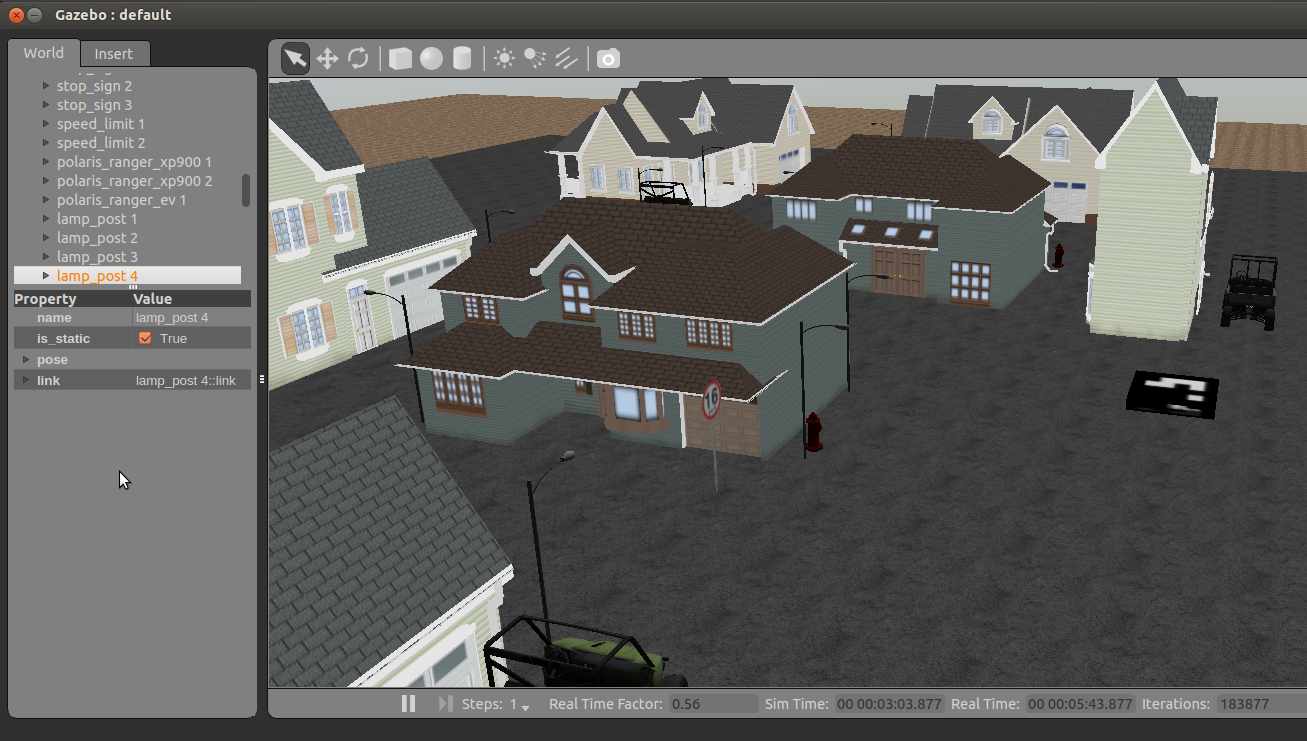
\includegraphics[width=0.5\textwidth]{imgs/gazeboworld.png}
				\caption{Mundo Gazebo.}
	\label{fig:MundoGazebo}
\end{figure}

\section{Entorno JdeRobot}
\hspace{1 cm} \'Este es el software principal con el que se ha trabajado, cuya web oficial es \underline{\url{www.jderobot.org}}. Se trata de un proyecto de software libre que se centra en la rob\'otica y en la visi\'on por computaci\'on. Este software cuenta con distintas herramientas como filtro de color o control de los diferentes robots, que ha permitido un continuo desarrollo desde el inicio. 


\subsection{Driver ArDroneServer}
\hspace{1 cm} \'Este es el servidor que permite comunicar nuestra aplicaci\'on con el drone. Tiene dos partes principales. Por un lado se encuentra el ArDrone SDK, el cual se comunica con el robot a\'ereo mediante WiFi. Por otro lado se encuentra el envoltorio C++, el cual se comunica con la aplicaci\'on mediante las interfaces ICE, permitiendo de esta forma la comunicaci\'on de nuestra aplicacio\'on con el cuadricoptero. 

\subsection{Plugin modelo de cuadricoptero Gazebo}
\hspace{1 cm} Plugin que permite tener un ArDrone2 de Parrot en el simulador. \'Este tiene distintos sensores con los que trabajar (sonar, IMU y c\'amara), adem\'as de contar con los distintos controles (cargar,iniciar, actualizar,despegue, velocidad y aterrizaje). Por otro lado, cuenta con la interfaz ICE para poder comunicar con los distintos elementos. 




\subsection{Herramienta UAVviewer}
\label{sec:uavviewer}
\hspace{1 cm} Esta herramienta permite el control del drone y obtener los datos de sus sensores. Su interfaz ICE tiene los drivers de C\'amara, Pose3D, CMDVel, NAVData y ArDrone\_Extra. 

\begin{figure}[H]
 \centering
  \subfloat[UAV\_Viewer Data]{
   \label{f:UAV_Viewer1}
    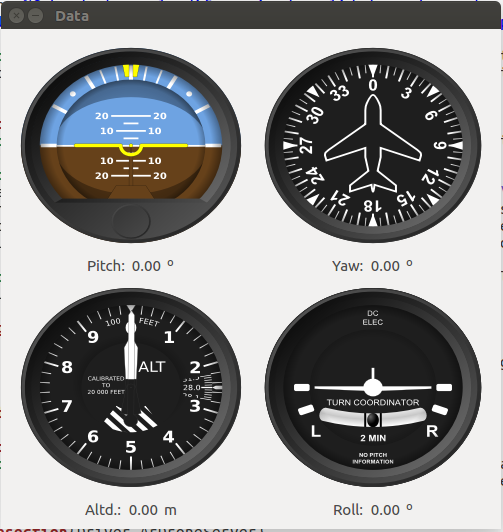
\includegraphics[width=0.29\textwidth]{imgs/UAV1.png}}
  \subfloat[UAV\_Viewer Tool]{
   \label{f:UAV_Viewer2}
    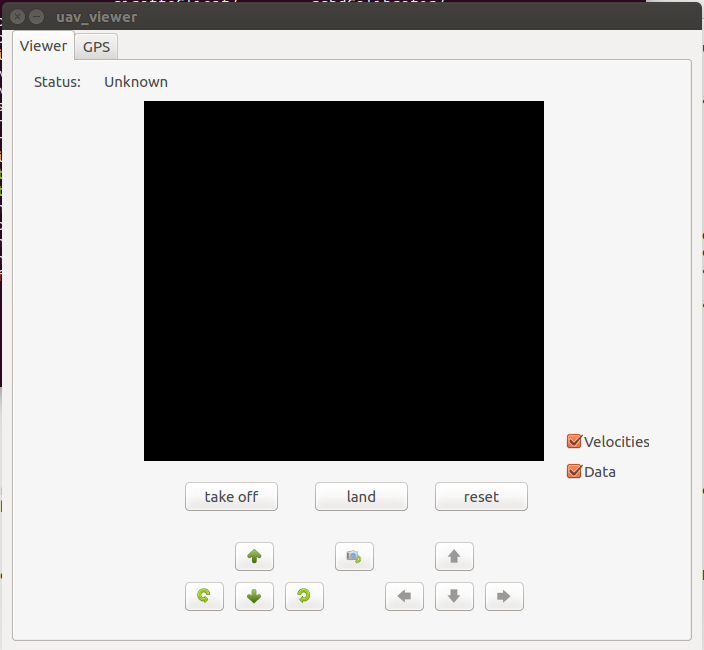
\includegraphics[width=0.33\textwidth]{imgs/UAV2.png}} 
  \subfloat[UAV\_Viewer Velocity]{
   \label{f:UAV_Viewer3}
    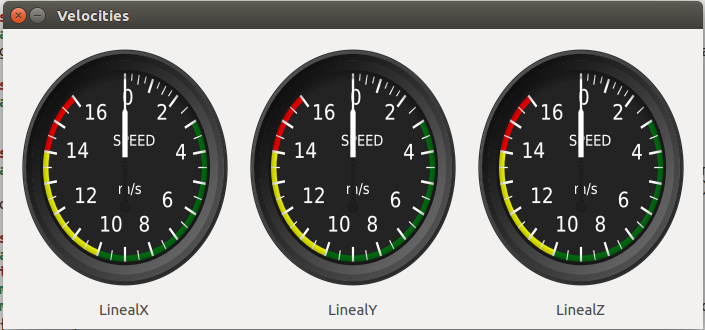
\includegraphics[width=0.25\textwidth]{imgs/UAV3.png}} 
 \caption{UAV viewer}
 \label{f:UAVViewerTotal}
\end{figure} 


\subsection{Herramienta ColorTuner}
\hspace{1 cm} Al inicio del proyecto era la herramienta \textit{ColorFilter}. Esta herramienta permite, a partir de una imagen o v\'ideo, trabajar en los distintos espacios de color (RGB, HSV, HSI...) y poder ir variando los par\'ametros m\'aximo y m\'inimo (entre 0 y 255) de cada uno para ver que colores cumplen las caracter\'isticas y cu\'ales no, viendose de esta forma, en otra imagen, s\'olo los colores que pasan este filtro dejando el resto como un fondo negro. 

%\subsection{JdeRobot Academy}
%\label{sec.JdeRobotAcademy}
%\hspace{1 cm} Con esta herramienta se ha trabajado en dos secciones.
\subsection{Pr\'actica choca-gira con aut\'omatas.}
\label{sec.JdeRobotAcademy}
\hspace{1 cm} De esta pr\'actica se ha obtenido la m\'aquina de estados, la cual permite crear diferentes estados, crear transiciones de unos a otros y marcar un estado u otro para saber en que punto se encuentra la aplicaci\'on. Con los siguienes comandos en el codigo python, la aplicaci\'on crea una m\'aquina (indicando el n\'umero de estados que tendra), añade un estado (indicando el nombre de este), añade una transici\'on (indicando origen, destino y el nombre) y marca el estado en el que se encuentra(indicando el numero del estado y TRUE para activarlo). 

\begin{lstlisting}[backgroundcolor=\color{yellow}]
 Machine(n)
 machine.addState(name) 
 machine.addTransition(orig, fin, name) 
 machine.setStateActive(n, flag) 
\end{lstlisting}


\begin{figure}[ht]
	\centering
		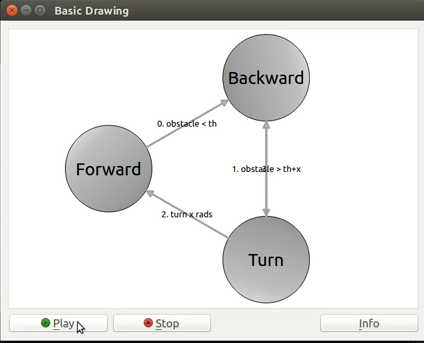
\includegraphics[width=9cm,height=7cm]{imgs/ChocaGiraAutomata.png}
		\caption{Diagrama de estados.}
	\label{fig:Diag_estados}
\end{figure}

Esta pr\'actica se encuentra en el GitHub de Jderobot Academy  \url{https://github.com/JdeRobot/Academy/tree/master/src/bump_and_go_py}


\subsection{Pr\'actica follow\_turtlebot.}
\hspace{1 cm} Al igual que UAV\_Viewer \ref{sec:uavviewer}, permite controlar el movimiento del drone, as\'i como ver los datos de sus sensores. A esta interfaz se le ha añadido la implementaci\'on de la maquina de estados obtenida de la pr\'actica de choca-gira, teniendo de esta forma el control del drone y poder visualizar el estado en el que se encuentra.


 \begin{figure}[H]
	\centering
		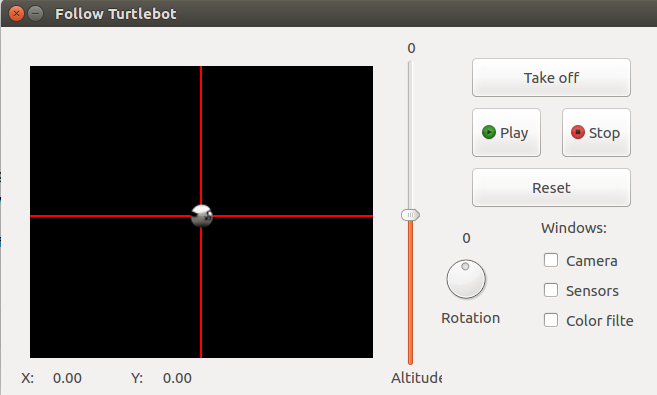
\includegraphics[width=0.5\textwidth]{imgs/follow_turtlebot.png}
		\caption{Follow Turtlebot.}
	\label{fig:FollowTurtlebot}
\end{figure}

\hspace{1 cm}Esta pr\'actica se encuentra en el GitHub de Jderobot Academy \url{https://github.com/JdeRobot/Academy/tree/master/src/follow_turtlebot}

\hspace{1 cm}Con la aplicaci\'on de la pr\'actica de follow\_turtleboot como interfaz, mas el componente añadido, el componente sobre el que se ejecuta el algoritmo est\'a compuesto por tres hilos. El primer hilo es el encargado de la ejecuci\'on del algoritmo. El segundo hilo es el encargado del interfaz gr\'afico para el control del drone, la c\'amara y los sensores. El tercer hilo es la ventana que permite ver el diagrama de estados. 
%\begin{itemize}
%\item 1ª Por una parte se ha utilizado para la pr\'actica de aut\'omatas. \'Esta permite crear un diagrama de estados para saber en cada momento en que punto del algoritmo nos encontramos.

%\begin{figure}[ht]
%	\centering
%		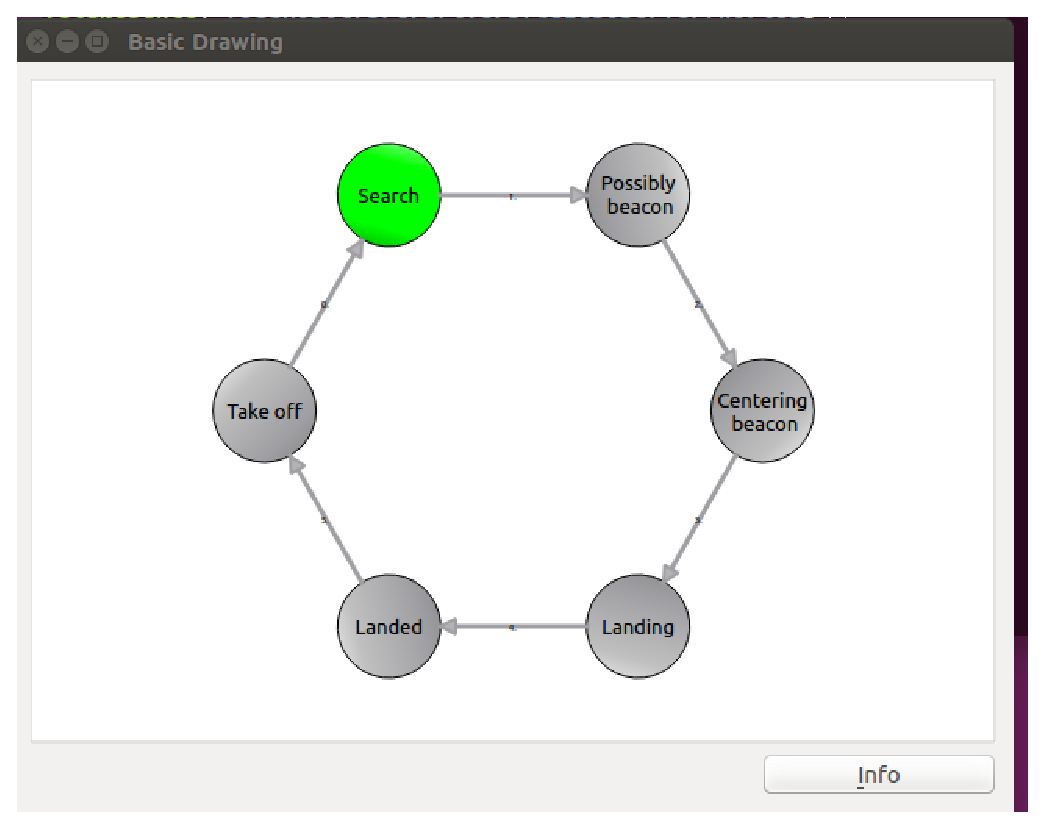
\includegraphics[width=0.3\textwidth]{imgs/states.eps}
%		\caption{Diagrama de estados.}
%	\label{fig:Diag_estados}
%\end{figure}

%\item 2ª Por otro lado se ha utilizado follow\_turtlebot, al igual que UAVviewer, permite controlar el drone y obtener los datos de sus sensores, adem\'as de poder indicar un algoritmo a ejecutar.
% \begin{figure}[H]
%	\centering
%		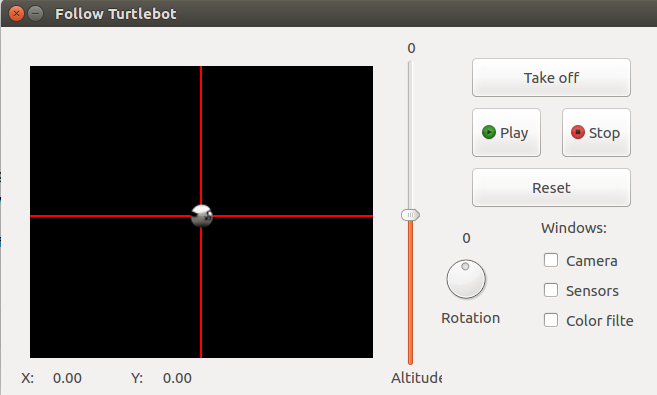
\includegraphics[width=0.5\textwidth]{imgs/follow_turtlebot.png}
%		\caption{Follow Turtlebot.}
%	\label{fig:FollowTurtlebot}
%\end{figure}


\end{itemize}

%En primer lugar se utiliz\'o \textit{color filter} para ver el funcionamiento de los filtros de color. Esta herramienta nos permite, a partir de una imagen o v\'ideo, trabajar en los distintos espacios de color (como puede ser RGB, HSV, HSI...) y poder ir variando los par\'ametros m\'aximo y m\'inimo (entre 0 y 255) de cada uno para ver que colores cumplen las caracter\'isticas y cuales no, viendose de esta forma, en otra imagen, s\'olo los colores que pasan este filtro dejando el resto como un fondo negro. 
%Una vez utilizada esta herramienta y realizamos pequeños algoritmos para ver que funcionaba igual un filtro propio que este filtro, pasamos a trabajar con otra llamada \textit{follow turtleboot}. \'Esta  nos permit\'ia manejar el dron, teniendo un cuadro que nos permite el movimiento en los ejes X e Y, una barra para realizar un cambio en la altura y un pequeño c\'irculo para que pudiera rotar sobre s\'i mismo. Por otro lado ten\'ia un bot\'on para aterrizaje y despegue y unos botones que permiten iniciar un algoritmo creado, de forma que podemos probar si lo programado funciona. Esta herramienta puede sacar tres cuadros diferentes, uno para la c\'amara, el cual nos da una imagen en directo de lo que est\'a transmitiendo el dron y nos da la opci\'on de elegir la c\'amara que queremos ver. El segundo, nos muestra las distintas propiedades del dron en ese momento como la orientaci\'on, altura o inclinaci\'on. Por \'ultimo, el \'ultimo cuadro es para el filtro de color. \'Este funciona cuando el algoritmo programado est\'a en marcha. En un primer momento como indica su nombre, nos permite trabajar con el filtro de color que hab\'iamos practicado antes sobre la otra herramienta, pero al final utilizamos \'este para realizar marcas sobre la imagen de las cosas que nos interesaban de \'esta, como puede ser encuadrar la baliza, la cruceta o pintar. 
%Por \'ultimo, a todo esto le hemos añadido un diagrama de estados, gracias a una pequeña aplicaci\'on desarrollar\'a a partir de \textit{visualHFSM}. nos permit\'ia crear un dibujo de los diferentes estados por los que deber\'ia pasar el dron, seg\'un lo que estuviera viendo en cada momento o la acci\'on concreta que estaba realizando. De esta forma se marca en el diagrama en el estado en el que se encuentra, pudiendo saber as\'i cual ser\'ia el siguiente estado esperado y viendo que funciona de forma correcta.


\section{Biblioteca OpenCV}
\label{sec:BibliotecaOpenCV} 
\hspace{1 cm} Esta librer\'ia tiene un conjunto de funciones que sirven para el procesamiento de im\'agenes y visi\'on computerizada, cuya web oficial es \underline{\url{https://opencv.org/}}. Est\'a programada en C++ y es un estandar de facto en la visi\'on artifical. Para el procesamiento de im\'agenes nos hemos apoyado principalmente sobre \'esta, trabajando en la versi\'on 3.1. Gracias a \'esta, al obtener la imagen que transmite el drone se puede tanto detectar objetos como aplicar cambios sobre ella, para marcar las zonas de interes o diferentes objetos. Permite la realizaci\'on de filtros de color, para eliminar objetos no deseados dependiendo el momento. Adem\'as permite el uso de operadores morfol\'ogicos (erosi\'on y dilataci\'on) gracias a los cuales se evitan imperfecciones en las im\'agenes como puede ser el ruido, que clasifica objetos inexistentes o de no inter\'es como objetos de inter\'es, as\'i como zonas importantes las detectaba como p\'ixeles de fondo. Tambi\'en han sido de gran utilidad funciones como \textit{drawContours} \'o \textit{findContours}, las cuales permiten encontrar los bordes de los objetos e indicar sobre una imagen final, con otro color, donde se encuentran dichos objetos. 



\begin{figure}[H]
 \centering
  \subfloat[Logo OpenCV]{
   \label{f:LogoOpenCV}
    
\includegraphics[width=0.29\textwidth]{imgs/opencv.png}}
  \subfloat[Procesamiento con OpenCV]{
   \label{f:OpenCVProcess}
    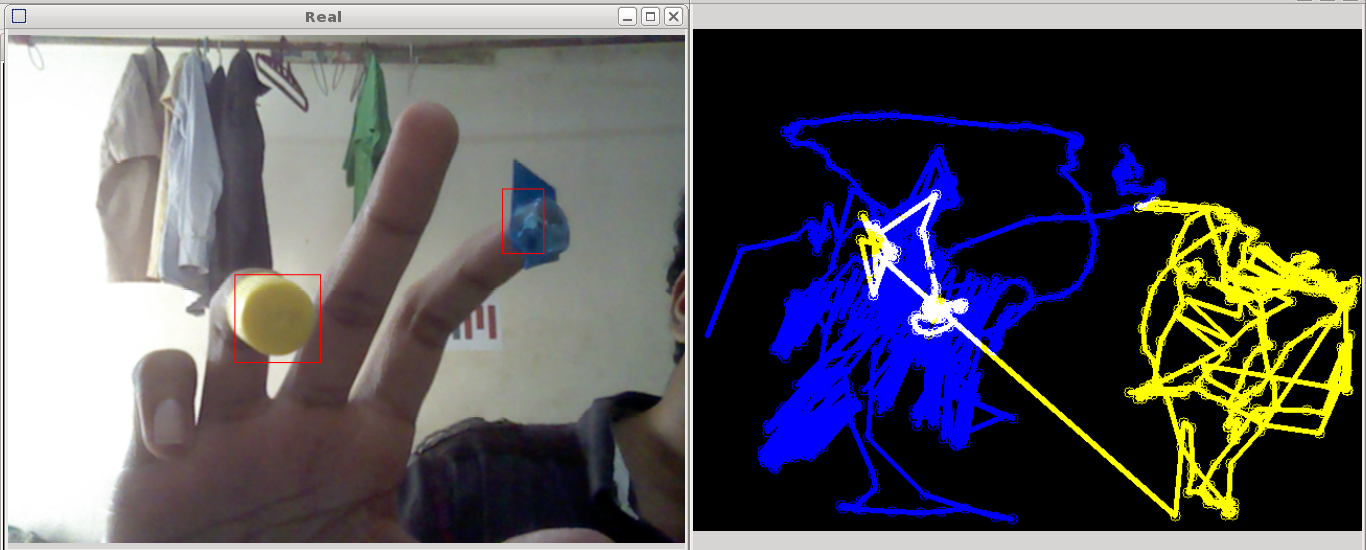
\includegraphics[width=0.7\textwidth]{imgs/opencvP.png}} 
 \caption{OpenCV}
 \label{f:OpenCV}
\end{figure} 










\lhead[]{CAPÍTULO \thechapter. ALGORITMO}
\chapter{Algoritmo}\label{cap.algoritmo}

\hspace{1 cm} En este cap\'itulo se describe el modo por el cual, con la infraestructura que se tiene, se llega a una soluci\'on para lo planteado en los objetivos. 

\hspace{1 cm} Este algoritmo tiene que permitir al drone despegar de forma controlada, realizar una navegaci\'on aut\'onoma para encontrar una baliza sobre la que aterrizar. La organizaci\'on de este cap\'itulo tiene primero una secci\'on de diseño, en el que se explica el funcionamiento del programa. Tras esto una secci\'on de percepci\'on para explicar los datos que se obtienen a trav\'es de los sensores, y para finalizar una secci\'on de control, para explicar los distintos movimientos del drone y de que dependen estos.

\section{Diseño}
\label{sec.Design}

\hspace{1 cm} El diseño de este algoritmo consta de un comportamiento reactivo de iteraciones continuas. Es un proceso basado en adquisici\'on-procesado-env\'io de datos. La adquisici\'on de los datos se realizan mediante los sensores del drone. Estos datos ser\'an transmitidos al dispositivo para que lo procese y tras estos se enviar\'an las instrucciones al drone para que este las ejecute. El sensor utilizado en este proyecto ha sido la c\'amara, y los movimientos del drone depender\'an de lo que esta capte en cada momento. 

\hspace{1 cm} Por otro lado, la parte es un aut\'omata finito de estados, el cual comienza en un estado inicial (despegue), y en funci\'on de lo que recibe a la entrada (imagen del sensor), realizar\'a el procesamiento necesario para producir la informaci\'on que enviar al drone, y en ocasiones le llevar\'a a pasar de un estado a otro. Destacar que este aut\'omata est\'a compuesto por 6 estados: despegando, buscando, posible baliza, centr\'andose en la baliza, aterrizando y aterrizado. A excepci\'on del primero, los dem\'as estados depender\'an de lo que detecte el drone en cada momento. El primer estado est\'a controlado por tiempo, pues son 10 segundos al iniciarse en los que el drone inicia el vuelo sobre una baliza y trata de estar centrado sobre \'esta, para as\'i tener un despegue controlado y evitar que el drone se mueva en caso de tener alguna deriva o haya factores externos que produzcan esto. Una vez transcurridos los 10 segundos se pasar\'a al estado de b\'usqueda e ir\'a pasando por los distintos estados hasta su aterrizaje. 

\begin{figure}[H]
	\centering
		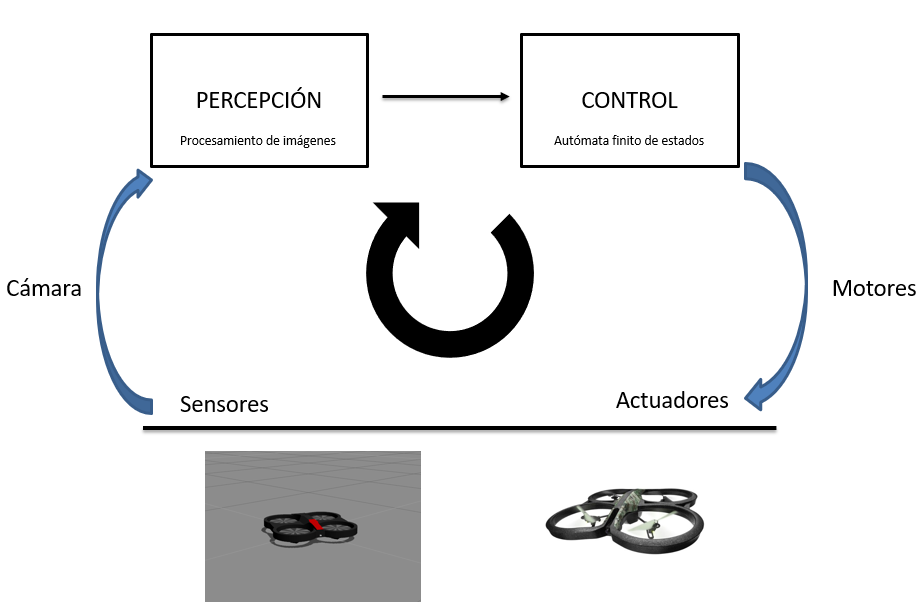
\includegraphics[width=0.75\textwidth]{imgs/esquema2.png}
	\label{fig:esquema_d}
\end{figure}

\hspace{1 cm} El lugar de aterrizaje del drone es una baliza previamente definida. Esta baliza es un cuadrado que en su interior tiene cuatro cuadrados, dos naranjas, y dos azules o verdes, dependiendo si se trabaja con el drone real o con el simulador. Esta baliza se ha elegido para que sea dif\'icil confundirla con otro objeto, pues de ser una baliza simple se podr\'ian confundir los colores. De esta forma lo que buscaremos ser\'a la cruceta que forman estos cuatro cuadrados y el punto central de \'esta. Por lo tanto, en lugar de un objeto en si lo que se busca es un objeto que tenga determinadas caracter\'isticas y patrones, algo que se puede detectar a diferentes alturas, distintas condiciones y situaciones.

\begin{figure}[H]
	\centering
		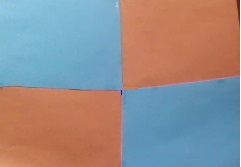
\includegraphics[width=0.3\textwidth]{imgs/baliza.jpg}
         \caption{Baliza utilizada para el drone real.}
	\label{fig:esquema_d}
\end{figure}


\hspace{1 cm} Por \'ultimo, para el control del drone con nuestro algoritmo se ha utilizado la herramienta follow\_turtlebot de JdeRobot Academy, explicada en \ref{sec.JdeRobotAcademy} . \'Esta aplicaci\'on tiene un interfaz gr\'afico de usuario (GUI) que permite controlar el drone y ver los datos de los distintos sensores, as\'i como la imagen que obtiene la c\'amara. Por otro lado cuenta con las interfaces ICE que permite la comunicaci\'on con el servidor, pudiendo as\'i recibir datos de sensores y motores, y enviar las instrucciones de velocidad necesarias en cada momento. La imagen de la aplicaci\'on se encuentra en la figura \ref{fig:FollowTurtlebot}


\section{Percepci\'on}

\hspace{1 cm} En \'esta secci\'on se va a tratar la obtenci\'on de la imagen de la c\'amara y el procesamiento que se realiza sobre \'esta. Gracias a lo que el drone ve en todo momento, sabe el punto del proceso en el que se encuentra y la informaci\'on que debe enviar. En primer lugar, se obtiene una imagen de entrada. Esta imagen es procesada con filtros de color y operadores morfol\'ogicos, obteniendo una imagen de salida. A partir de los datos de \'esta imagen, se detecta si hay objetos de inter\'es o no, y por tanto se env\'ia unas instrucciones u otras al drone. 


\subsection{Pre-procesado}

\hspace{1 cm} Una vez tenemos la imagen de entrada, hay que detectar la informaci\'on de interes que nos aporta. 
 
\hspace{1 cm} En primer lugar, la imagen que est\'a en RGB se transforma a HSV, para que sea m\'as facil su interpretaci\'on, ya que en lugar de trabajar en funci\'on de tres colores (rojo, verde y azul), se trabaja en funci\'on de tres par\'ametros (tono, saturaci\'on y valor). De \'esta forma, se depende menos de la luz que haya en cada momento y en cada lugar. En el filtro, a cada uno de los par\'ametros se le asigna un rango de valores entre 0 y 255. La herramienta colorTuner permite, a partir de una imagen de entrada, dar valores a estos par\'ametros, viendo que objetos cumplen estos requisitos y dejandolos en primer plano, y cuales no, dejando estas zonas en negro como p\'ixeles de fondo. Una vez se obtienen estos valores se añaden al filtro, obteniendo a la salida una imagen que solo muestra los objetos de los colores de inter\'es. 

\hspace{1 cm} El siguiente c\'odigo es un ejemplo de como, a partir de una imagen de entrada en RGB, se transforma a HSV y se filtran los objetos de color naranja. 

\begin{lstlisting}[backgroundcolor=\color{yellow}]
hsv = cv2.cvtColor(input_image, cv2.COLOR_BGR2HSV)
lower_orange = np.array([100,100,80], dtype=np.uint8)
upper_orange = np.array([150, 255,255], dtype=np.uint8)
maskOrange = cv2.inRange(hsv, lower_orange, upper_orange)
maskRGBOrange = cv2.bitwise_and(input_image,input_image, mask= maskOrange)
\end{lstlisting}


\hspace{1 cm} En caso de trabajar sobre simulador, con esto se obtiene a la salida una imagen bastante parecida a la deseada, debido a la pureza e los colores. Sin embargo, al trabajar sobre im\'agenes reales, la imagen de salida de este filtro a\'un tiene ruido y objetos de inter\'es imperfectos. Para arreglar esto se utilizan los operadores morfol\'ogicos, que eliminan estas imperfecciones. Una breve explicaci\'on de los utilizados es la siguiente: 

\begin{itemize}
	\item \textbf{Erosi\'on:} Dada una imagen y un elemento estructural, la erosi\'on es el conjunto de los elementos \textit{x} para los cuales el elemento estructural trasladado por \textit{x} est\'a contenido en la imagen. 
	\newline\hspace{1 cm} Aplicaci\'on: Cuando un p\'ixel que parece pasar el filtro, pero los elementos de su alrededor (en concordancia con el elemento estructurante) no lo pasan, \'este pasa a ser parte del fondo. 
	\item \textbf{Dilataci\'on:} Transformaci\'on dual a la erosi\'on. El resultado de \'esta es el conjunto de elementos tal que al menos alg\'un elemento del conjunto estructurante esta contenido en \textit{x}, cuando el elemento estructurante se desplaza sobre \textit{x}
	\newline\hspace{1 cm} Aplicaci\'on: p\'ixeles que parecen de fondo, pasan a ser de la figura si est\'an cerca de p\'ixeles que pasan el filtro.
	\item \textbf{Cierre:} Se trata de realizar una dilataci\'on en la imagen seguida de una erosi\'on.
	\item \textbf{Apertura:} Se trata de realizar la erosi\'on en una imagen seguida de una dilataci\'on.
\end{itemize}


\hspace{1 cm} De esta forma, al obtener una imagen sin apenas ruido, evitando as\'i que objetos de no inter\'es los detecte como tal y que los objetos de interes los trate como p\'ixeles de fondo. Una im\'agen en la que se observa la realizaci\'on de un filtro de color y el uso de operadores morfol\'ogicos es la siguiente:

\begin{figure}[ht]
	\centering
		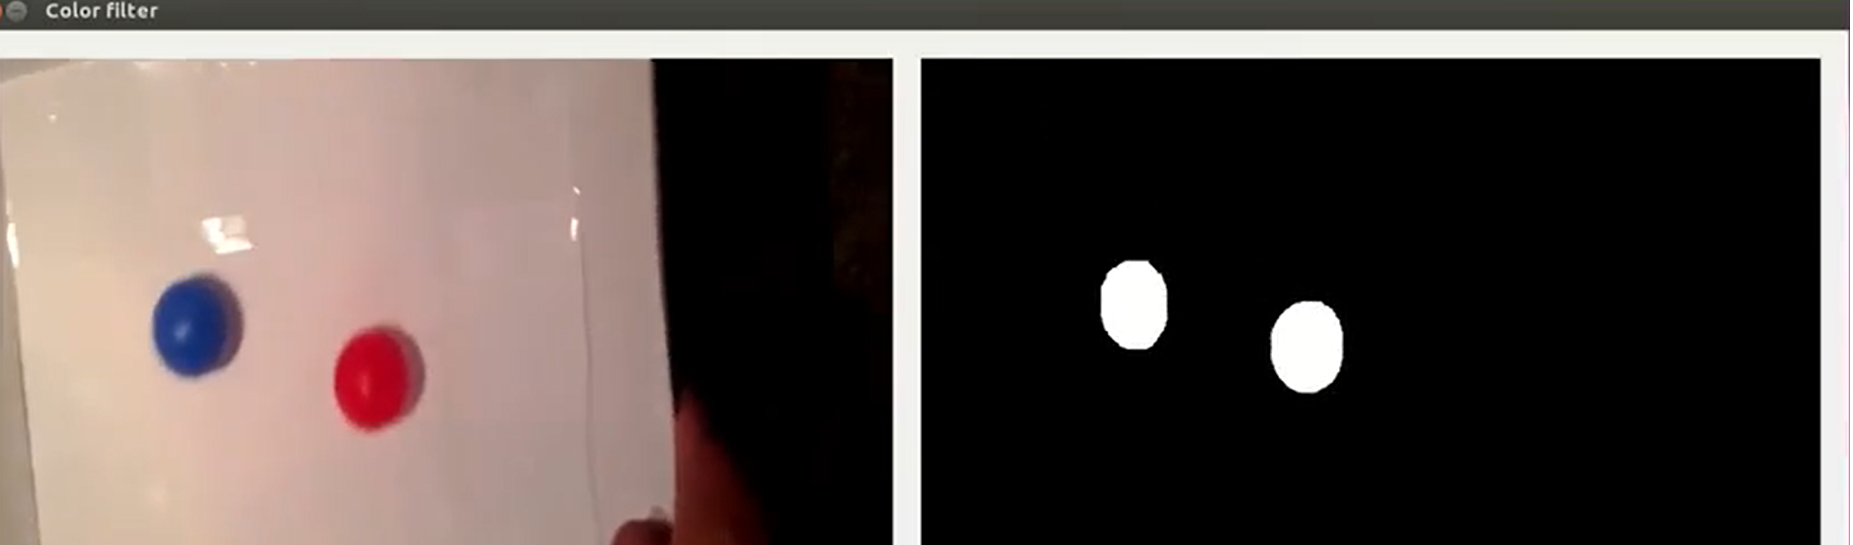
\includegraphics[width=0.8\textwidth]{imgs/colorfilter.eps}
	\label{fig:E_Imagen_baliza}
\end{figure}


\hspace{1 cm} El siguiente fragmento de c\'odigo, muestra como se define la matriz a partir de la cual se realizar\'an las operaciones oportunas, y despues se realizan la erosi\'on y la dilataci\'on.
\begin{lstlisting}[backgroundcolor=\color{yellow}]
kernel = np.ones((3,3),np.uint8)
maskRGBOrange = cv2.erode(maskRGBOrange,kernel,iterations = 4)
maskRGBOrange = cv2.dilate(maskRGBOrange,kernel,iterations = 3)
\end{lstlisting}


\subsection{Detecci\'on de la baliza}
\hspace{1 cm} Una vez se obtienen los colores de los objetos de inter\'es, hay que buscar el objeto deseado. Para \'esto hay que buscar el punto de intersecci\'on entre los cuatro cuadrados de la baliza. Para ello, los pasos a realizar son los siguientes:

\begin{enumerate}
	\item Para la imagen de entrada se hacen dos filtros de color, uno por cada color de la baliza.
	\item De cada imagen se obtienen el n\'umero de objetos, las \'areas y los contornos. En cada objeto se obtiene el valor de su \'area, en caso de ser menor de un valor determinado, \'este se descarta. En caso de tener ese \'area o mayor, se crea una imagen negra, se pintan los contornos del objeto sobre esta con un valor RGB(0,1,0) y se dilatan. De esta forma, tendremos tantas im\'agenes como objetos. 
	\item Se suman las im\'agenes obtenidas, por lo tanto, sobre una imagen negra final se pintaran los contornos dilatados de todos los objetos. Cada contorno se pintar\'a con un valor RGB(0,1,0), por lo tanto en el caso de que varios objetos coincidan sumar\'an sus valores. Con esto conseguiremos que el punto donde interseccionen cuatro objetos tenga un valor (0,4,0), y por tanto \'este ser\'a el centro de la cruceta.
	
\hspace{1 cm}El siguiente fragmento de c\'odigo muestra la creaci\'on de una imagen por objeto, la dilataci\'on de los contornos y la suma final de las im\'agenes:

\begin{lstlisting}[backgroundcolor=\color{yellow}]
f = []
i=0
imgray2 = cv2.cvtColor(maskRGBOrange,cv2.COLOR_BGR2GRAY)
ret,thresh = cv2.threshold(imgray2,255,255,255)
_,contours, hierarchy = cv2.findContours(thresh,cv2.RETR_TREE,
                                          cv2.CHAIN_APPROX_SIMPLE)
\'areas = [cv2.contour\'area(c) for c in contours]
for extension in \'areas:
    if extension > 100:
    img = np.zeros((y_img*2,x_img*2,3), np.uint8)
        actual = contours[i]
        approx = cv2.approxPolyDP(actual,0.05*cv2.arcLength(actual,True),
                                                                       True)
        cv2.drawContours(img,[actual],0,(0,30,0),12)
        f.append(img)
        i=i+1
			
kernel = np.ones((3,3),np.uint8)
if(len(f)>0):
    f[0] = cv2.dilate(f[0],kernel,iterations = 4)
    show_image2=f[0]
    for k in range(len(f)-1):
        f[k+1] = cv2.dilate(f[k+1],kernel,iterations = 4)
        show_image2=show_image2+f[k+1]
		
\end{lstlisting}


	\item A partir de la imagen final, se pasar\'a un filtro RGB que filtre los valores mayores a RGB(0,3,0), por lo tanto el \'unico valor que no se eliminar\'a sera el del centro de la cruceta.

	\item Sobre la imagen obtenida, utilizando la funci\'on drawcontours, obtenemos la situaci\'on de estos y p\'ixeles, teniendo as\'i la situaci\'on de la cruceta, y con estos valores se puede marcar el centro de la baliza sobre la imagen real. En caso de haber filtrado la intersecci\'on de dos objetos en lugar de cuatro en el apartado anterior, se podr\'ian marcar tambi\'en posibles objetos de inter\'es, como puede ser la baliza completa. 

\hspace{1 cm}En el siguiente fragmento de c\'odigo se muestra, como a partir de la imagen de la suma de objetos, se calcula la posici\'on de la cruceta y se marcan sobre la imagen. En \'este caso, para que se obtuviera una imagen m\'as clara, a los bordes de los objetos se les da un valor de 30, por lo tanto la intersecci\'on de 3 objetos tendr\'a un valor RGB(0,90,0) y de 4 objetos un valor RGB(0,120,0).

\begin{lstlisting}[backgroundcolor=\color{yellow}]
lower_green = np.array([0,80,0], dtype=np.uint8) 
upper_green = np.array([0, 140,0], dtype=np.uint8) 
maskSHI = cv2.inRange(show_image2, lower_green, upper_green)
show_image2 = cv2.bitwise_and(show_image2,show_image2, mask= maskSHI)

compare_image = np.zeros((y_img*2,x_img*2,3), np.uint8)
diff_total = cv2.absdiff(compare_image, show_image2)

imagen_gris = cv2.cvtColor(diff_total, cv2.COLOR_BGR2GRAY)
_,contours,_ = cv2.findContours(imagen_gris,cv2.RETR_EXTERNAL, 
                                             cv2.CHAIN_APPROX_SIMPLE)

positionX=-1
positionY=-1
for c in contours:
    if(cv2.contour\'area(c) >= 0):
        posicion_x,posicion_y,ancho,alto = cv2.boundingRect(c) 
        cv2.rectangle(show_image,(posicion_x,posicion_y),
                    (posicion_x+ancho,posicion_y+alto),(0,0,255),2)
        positionX= (posicion_x+posicion_x+ancho)/2
        positionY= (posicion_y+posicion_y+ancho)/2
\end{lstlisting}

\end{enumerate}

\hspace{1 cm} En el conjunto de im\'agenes siguiente, se observa la imagen de entrada, en la cual esta marcado el centro de la baliza y el objeto de inter\'es, y la suma de los bordes de los distintos objetos, siendo los puntos donde m\'as contornos se cruzan de un color m\'as intenso. 

\begin{figure}[H]
 \centering
  \subfloat[Imagen real]{
   \label{f:imagen real}
    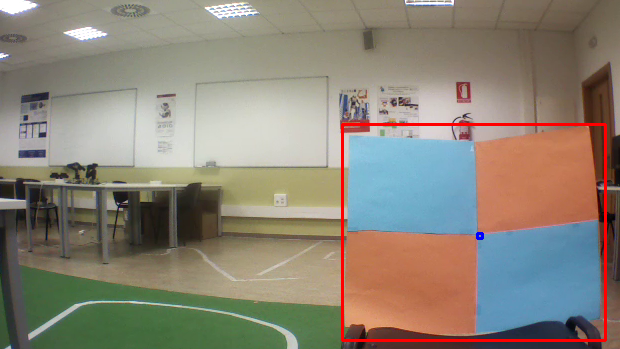
\includegraphics[width=0.29\textwidth]{imgs/k_beacon21.png}}
  \subfloat[Suma de objetos]{
   \label{f:sumaobjetos}
    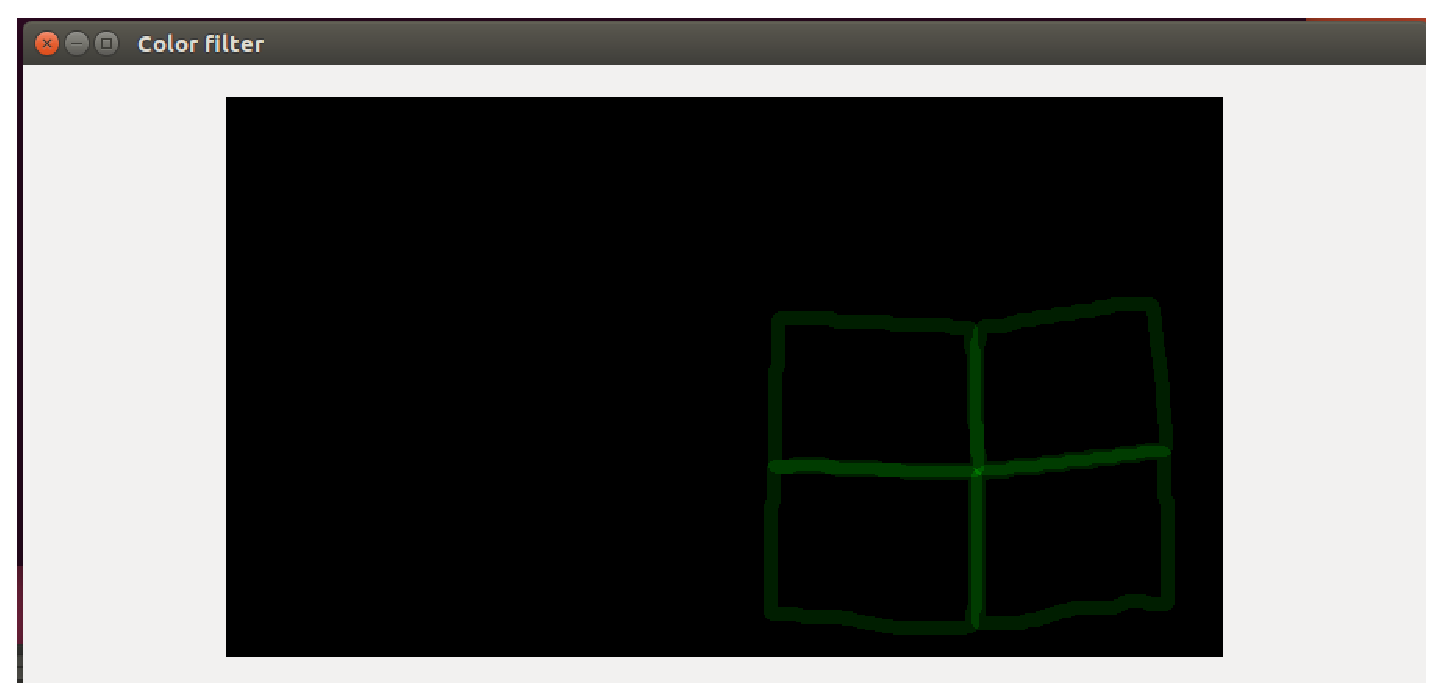
\includegraphics[width=0.33\textwidth]{imgs/k_Beacon1.eps}} 
 \caption{Procesamiento de imagen de la baliza}
 \label{f:ColorFilterTotal}
\end{figure} 



\section{Control}
\label{sec.control}

\hspace{1 cm} En \'esta secci\'on se explica el control sobre el drone en funci\'on del momento en el que se encuentra y la imagen que se obtiene. Se puede dividir \'esta secci\'on en tres partes:
despegue, b\'usqueda y aterrizaje.


\subsection{Despegue}

\hspace{1 cm} Esta fase est\'a controlada por tiempo. Son los primeros diez segundos del algoritmo, y en ellos el drone despega de forma controlada. Esta fase ser\'a "`Take off"' en el aut\'omata de estados. Para ello se sit\'ua el drone sobre una baliza sobre la cual tiene que estabilizarse. De esta forma, al despegar detecta \'esta y trata de centrarse, evitando as\'i que se desv\'ie por factores externos y qued\'andose en la situaci\'on correcta. Debido a que el drone va a despegar sobre la baliza, el control en esta parte es un control proporcional, para evitar que tenga que hacer m\'ultiples operaciones, por tanto sea mas r\'apido el algoritmo, y suficiente para ser controlado.



\subsection{B\'usqueda}
\hspace{1 cm} Esta fase comenzar\'a cuando finalicen los diez segundos de despegue. El drone comenzar\'a a navegar de forma aut\'onoma en b\'usqueda de una baliza sobre la cual aterrizar. Para ello comenzar\'a un algoritmo en espiral, estado "`Search"', de forma que ir\'a rastreando la zona ampliando su giro de forma continua, hasta que detecte una posible baliza. En el momento que la detecte, pasar\'a al estado "`Possibly beacon"' e intentar\'a centrarse sobre ella. Si tras un n\'umero previamente definido de iteraciones, no se trata de una b\'aliza, continuar\'a el algoritmo de b\'usqueda en el punto donde se hab\'ia quedado, siguiendo con la amplitud de las espirales a la que se hab\'ia llegado. Pero en caso de serlo pasar\'a al estado "`Centering beacon"', haciendo que coincida el centro de la baliza con el centro de la imagen de la c\'amara. Para realizar el movimiento de centrarse en la baliza se ha utilizado un control PD (progresivo y derivativo). Esto se debe a que s\'olo con el control progresivo, se produc\'ia una gran diferencia de velocidad y el drone cambiaba sus giros de forma muy brusca, lo que le llevaba a desestabilizarse y perder con facilidad la baliza. El algoritmo del control PD es de la siguiente forma:

\begin{itemize}
\item Por una parte, se tiene el control progresivo. Para \'este se obtiene por un lado el centro de la imagen, y por otro lado el centro de la cruceta o del objeto de interes, segun el punto del algoritmo. Se calcula la diferencia entre el centro de la imagen y el centro de referencia, obteniendo as\'i el error, y como resultados, para el eje x $\Delta_x$,  y para el eje y $\Delta_y$. Estos valores, se multiplican por una constante que sirve para adaptar el resultado a la velocidad del drone. La formula de este control es la siguiente:  \[\Delta_x = centroimagen_x - centroobjeto_x\]   \[\Delta_y = centroimagen_y - centroobjeto_y\]  \[ P_x = \Delta_x * 0.01\]  \[P_y = \Delta_y * 0.01\]




\item Por otro lado, est\'a el control derivativo. Para este caso, al tratarse de iteraciones, se trabaja con las diferentes muestras de cada iteración. Se obtiene el error de la iteraci\'on actual y de la iteraci\'on anterior para ambos ejes, y se resta el error anterior al actual: \[\Delta_d_i_f_e_r_e_n_c_i_a_x =  \Delta_x [n] - \Delta_x [n-1] \] \[\Delta_d_i_f_e_r_e_n_c_i_a_y =  \Delta_y [n] - \Delta_y [n-1] \]

\end{itemize}

\hspace{1 cm} Una vez se ha obtenido esto, se envian las instrucciones de velocidad al drone, utilizando el comando:
\begin{lstlisting}[backgroundcolor=\color{yellow}]
vely = (y_img-positionX)                        
velx = (x_img-positionY)

vytot= vely*0.01 
vxtot= velx*0.01

velxa=1-abs(xanterior-velx)/50 #10
if(velxa<0.1):    
    velxa=0.1

velya=1-abs(yanterior-vely)/50 #10
if(velya<0.1):
    velya=0.1
self.cmdvel.sendCMDVel(vytot*velya,vxtot*velxa,0,0,0,0) 
\end{lstlisting}
	

 %$\\ Calculo \Delta_x : \[\Delta_x = centroimagen_x - centroobjeto_x\] \\ Calculo \Delta_x : \[\Delta_y = centroimagen_y - centroobjeto_y\] \\ Calculo del control proporcional P_x : \[ P_x = \Delta_x * 0.01\] \\ Calculo del control proporcional P_y : \[P_y = \Delta_y * 0.01\] 




%\hspace{1 cm} Esta fase comenzar\'a cuando finalicen los diez segundos de despegue. El drone comenzar\'a a navegar de forma aut\'onoma en b\'usqueda de una baliza sobre la cual aterrizar. Para ello comenzar\'a un algoritmo en espiral, estado "`Search"', de forma que ir\'a rastreando la zona ampliando su giro de forma continua, hasta que detecte una posible baliza. En el momento que la detecte, pasar\'a al estado "`Possibly beacon"' e intentar\'a centrarse sobre ella. En caso de no tratarse de la baliza, continuar\'a con el algoritmo de b\'usqueda, pero en caso de serlo pasar\'a al estado "`Centering beacon"', haciendo que coincida el centro de la baliza con el centro de la imagen de la c\'amara. Para realizar el movimiento de centrarse en la baliza se ha utilizado un control PID (progresivo, integral y derivativo). Esto se debe a que s\'olo con el control progresivo, se produc\'ia una gran diferencia de velocidad y el drone cambiaba sus giros de forma muy brusca, lo que le llevaba a desestabilizarse y perder con facilidad la baliza.  Este control se basa en derivar el error con respecto al tiempo y multiplicarlo por una constante. Dado que nuestro algoritmo ejecuta una vez cada cierto tiempo y no esta continuamente pasando por este punto, podemos considerar que se trata de un sistema en tiempo discreto, y por tanto en lugar de trabajar con derivadas trabajaremos con sumatorios. De esta forma, para añadir un control derivativo se realiza una operaci\'on que depende de la velocidad anterior y la que tenemos ahora: \[v_{derivativa} =1-(v_{anterior}-v_{nueva})/50 \] 

\hspace{1cm}Para evitar que el valor sea 0 y al multiplicarlo por el valor progresivo se quede en el sitio, en caso de ser un valor menor a 0.1 se iguala a \'este. Este resultado lo multiplicamos a la velocidad final, y lo que conseguimos es que si el valor entre dos velocidades continuas es muy alto, \'este se aten\'ue de forma que el drone no cambie mucho y vaya oscilando, sino que lleve una velocidad m\'as continua a la hora de acelerar o frenar.  

El siguiente fragmento de c\'odigo consigue que el drone se mueva realizando espirales:

\begin{lstlisting}[backgroundcolor=\color{yellow}]
self.cmdvel.sendCMDVel(1.8+wSearch,0,0,0,0,1.5 - wSearch)
numVuelta=numVuelta+1
if(numVuelta==100):
    timerW=timerW+(timerW/8)
    numVuelta=0
    if(wSearch<1):
        wSearch=wSearch+0.2
\end{lstlisting}

\hspace{1 cm} El esquema de este control es el siguiente:
\begin{figure}[ht]
	\centering
		
\includegraphics[width=1\textwidth]{imgs/esquemapd2.png}
	\label{fig:Esquema_control}
\end{figure}


\hspace{1cm} Para visualizar el diagrama de estados, se tuvieron que añadir dos paquetes del GUI de JdeRobot, uno que permit\'ia abrir otra ventana y otro que permit\'ia añadir estados y transiciones entre ellos. Para marcarlo, siendo el numero que aparece el numero del estado que queremos marcar, val\'ia con la siguiente linea de c\'odigo:

\begin{lstlisting}[backgroundcolor=\color{yellow}]
self.machine.setStateActive(2, True)
\end{lstlisting}
	
\hspace{1cm}La imagen del diagrama que ver\'iamos durante la ejecuci\'on se encuentra en \ref{fig:Diag_estados}.

\subsection{Aterrizaje}

\hspace{1 cm} Esta fase es un aterrizaje controlado. Una vez el drone se ha centrado sobre la baliza comienza a descender de forma constante , cambiando el estado a "`Landing"'. Una vez el \'area es menor a 19272135.0, se manda la instrucci\'on de parar motores. En este momento el drone desciende hasta posarse en el suelo, entonces para los motores y el estado cambia a "`Landed"'. La raz\'on de ir descendiendo poco a poco hasta detectar determinado \'area, es por si la baliza est\'a lejos del drone, puede interferir alg\'un objeto moment\'aneamente o darse alg\'un factor externo que altere la posici\'on del drone respecto de la baliza, y al enviar la instrucci\'on de aterrizar se perder\'ia este control. El \'area elegido es porque en ese momento la baliza ocupa pr\'acticamente por completo la imagen, y si se le indicara al drone que siguiera descendiendo las corrientes que se producir\'ian con el suelo podr\'ian afectarle y desviar su trayector\'ia, pudiendo perder la referencia.


\hspace{1 cm} Una vez finalizada la descripci\'on del algoritmo completo, un esquema del control completo es el siguiente:
\begin{figure}[ht]
	\centering
		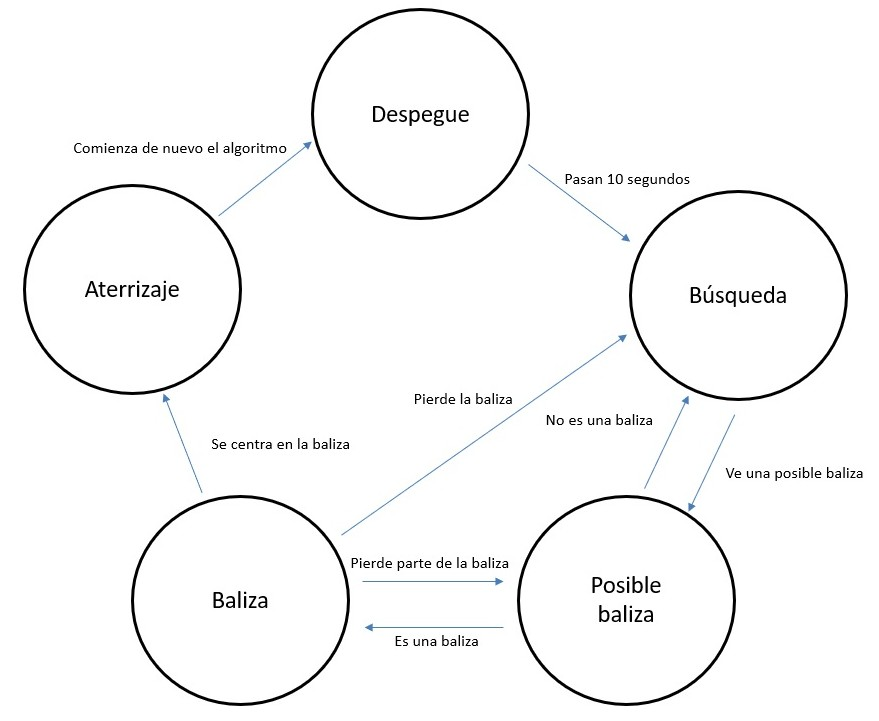
\includegraphics[width=1\textwidth]{imgs/EsquemaAlgoritmo.jpg}
	\label{fig:Esquema_control}
\end{figure}


%Esta fase es un aterrizaje controlado, en el cual, una vez que el drone se ha centrado sobre la baliza comienza a descender, cambiando su estado a "`Landing"', y una vez el \'area de la baliza es suficiente, como para detectar que el drone est\'a muy pr\'oximo a ella, se env\'ia la instrucci\'on land, aterrizando de \'esta forma el drone, siendo aqu\'i su estado "`Landed"'. El hecho de enviarse la orden de aterrizar cuando se est\'a a una distancia cercana a la baliza es porque esta instrucci\'on es a ciegas, una vez que se env\'ia el drone solo se encarga de descender hasta que nota que est\'a sobre un lugar sobre el cual posarse. Por lo tanto si se env\'ia esta orden a una distancia lejana, el drone puede perder la referencia y aterrizar en otro sitio. 
























\lhead[]{CAPÍTULO \thechapter. EXPERIMENTOS}
\chapter{Experimentos}\label{cap.experimentos}
\hspace{1cm} En este cap\'itulo se van a comentar las distintas pruebas realizadas tanto con el drone real como en la simulaci\'on, las cuales validan cada fase del proyecto y la soluci\'on final. Tambi\'en estas pruebas han servido para depurar mientras se desarrollaba. 

\hspace{1cm} Para organizar las distintas pruebas, se va a hablar sobre la parte de percepci\'on. Tras esto se comentar\'a por separado cada una de las partes del algoritmo de navegaci\'on (despegue, b\'usqueda y aterrizaje), para terminar con una ejecuci\'on t\'ipica del algoritmo completo.

\hspace{1cm} En los experimentos realizados se han apreciado las diferencias importantes que hay entre trabajar en el entorno simulado y en el real. Primero, en el entorno simulado los colores son puros ideales y m\'as f\'aciles de detectar, sin embargo en el entorno real debido a luces y sombras un color puede verse m\'as o menos n\'itido, adem\'as de ser m\'as dif\'icil aislarlo del resto. Segundo, las velocidades a los motores a aplicar sobre uno y otro son distintas, pues en el entorno simulado se le puede dar una mayor velocidad que trabajar\'a sin problemas. Por el contrario, en el real una velocidad alta y un movimiento brusco puede llevar a desestabilizarlo. Tercero, en el drone real interviene tambi\'en el factor de la bater\'ia, en funci\'on de la carga que tuviera \'esta el drone aterrizaba con m\'as o menos fuerza y realizaba movimientos m\'as o menos fluidos. A partir del 30\% de bater\'ia no permit\'ia al drone realizar todos los movimientos, y en algunas ocasiones perd\'ia altura, aunque despu\'es volv\'ia a ganarla. 

\hspace{1cm} Los experimentos reales se han realizado con 3 ArDrone2 de Parrot distintos, entre los que se han apreciado comportamientos distintos pese a ser el mismo modelo del mismo fabricante. Se debe a que alguno ten\'ia mas deriva que los otros o que los movimientos eran mas bruscos seg\'un el drone.


\section{Percepci\'on de la baliza}\label{sec:percepcion}
%%QUE OBJETO DETECTAR???
\hspace{1cm} Para las pruebas de esta secci\'on hay que tener en cuenta que objeto detectar. Es un cuadrado con cuatro cuadrados dentro, dos de color naranja, y otros dos de color azul (trabajando con el drone real) o verde (si se trabajaba en un entorno simulado). 

%\hspace{1cm} Los primeros test se realizaban en el entorno simulado, al principio detectando ambos colores y viendo que se trataba de 4 objetos distintos. Despu\'es se comenzaron los test con el algoritmo final, viendo que los cuatro cuadrados formaban una cruceta y detectaba \'esta en la imagen, para as\'i poder centrarse. Dependiendo de los distintos estados del algor\'itmo, cuando ve\'ia una parte de la baliza la detectaba y marcaba como posible objeto, en caso de tratarse de la baliza completa la marcaba como tal. 


\hspace{1cm} Para verificar el funcionamiento de los filtros de color se realizaron tests en los cuales se detectaban por separado los colores de la baliza y se contaba el n\'umero de objetos. Para verificar que los objetos que se detectaban eran la baliza deseada, se pasaba por dos fases. Para una posible baliza, se marcaba el objeto en el interfaz gr\'afico. En caso de que se detectara la cruceta de los 4 cuadrados, se señalaba \'esta sobre la imagen y la baliza completa, como muestra la figura \ref{f:Deteca_objeto}.

\begin{figure}[H]
 \centering
  \subfloat[Percepci\'on posible objeto]{
   \label{f:Posible objeto}
    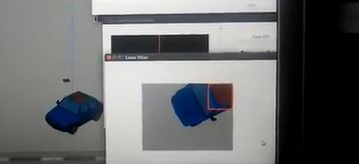
\includegraphics[width=0.4\textwidth]{imgs/perception1.jpg}}
  \subfloat[Detecta objeto]{
   \label{f: Deteca_objeto}
    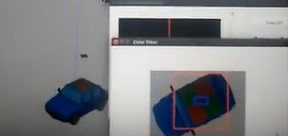
\includegraphics[width=0.4\textwidth]{imgs/perception2.jpg}} 
 \caption{Drone detectando objeto en escenario simulado.}
 \label{f:Drone detecta objeto. }
\end{figure} 

%\hspace{1cm} Una vez se realizaron \'estos con \'exito, pasaron a realizarse las pruebas con el drone real. Las primeras pruebas eran con el drone quieto y situando las balizas en distintas posiciones y viendo que las detectaba. Tras esto con el drone volando se hicieron pruebas, viendo que cuando se situaba la baliza debajo de este era capaz de detectarla. 

\hspace{1cm} Para realizar las pruebas en un entorno real se pon\'ia el drone en una posici\'on fija y se iba moviendo la baliza sobre distintas posiciones de la c\'amara y viendo si las detectaba o no. Para observar lo que detectaba se marcaba en la interfaz gr\'afica en color azul el centro de la cruceta y con rojo los posibles objetos, coincidiendo con la baliza completa, como muestra la figura \ref{fig:Detectando_baliza_real}.

\begin{figure}[H]
	\centering
		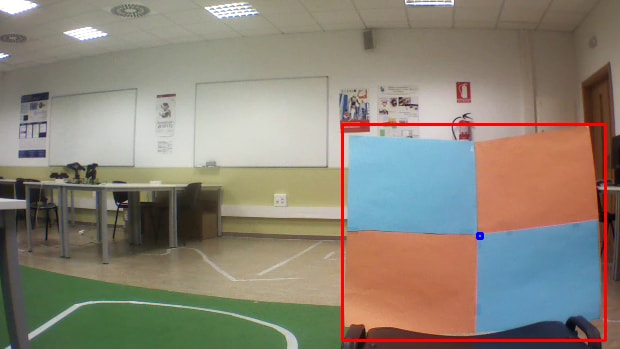
\includegraphics[width=0.55\textwidth]{imgs/k_beacon21.jpg}
		\caption{Detectando baliza real.}
	\label{fig:Detectando_baliza_real}
\end{figure}


\hspace{1cm} La parte de la percepci\'on es satisfactoria, pues se ha conseguido una detecci\'on robusta. Apenas hay falsos negativos(no detectar una baliza existente), y tampoco falsos positivos(detectar como baliza algo que no lo es). Adem\'as, el algoritmo se ha probado en diferentes ambientes con distinta luminosidad. Es importante tambi\'en el tipo de baliza elegida a detectar, ya que es un objeto dif\'icil de confundir con otros.


\section{Despegue}

%\hspace{1cm} Las primeras pruebas del despegue sobre el simulador fueron las mas sencillas. Esto se debe a que se trata de un entorno ideal en el cual el drone no tiene deriva ni se dan otros factores externos. Las pruebas consist\'ian en despegar el drone y que este se centrara sobre la baliza, aunque tambi\'en se prob\'o a despegar el drone sobre el coche con la baliza y mover el coche para ver que el drone le iba siguiendo. Esta parte se decidi\'o implementar porque el drone ten\'ia una deriva que le llevaba a desplazarse hacia atr\'as cuando ten\'ia que estar en el sitio. Cuando se hicieron las primeras pruebas de esto, se vi\'o que el drone siempre despegaba en esta direcci\'on y hab\'ia un dos segundos en los que no se pueden controlar sus movimientos, por tanto hab\'ia que contar con este desplazamiento.

\hspace{1cm} Para verificar el despegue en un entorno simulado, las pruebas que se realizaron fueron fructiferas (figuras \ref{fig:Despegue sobre la baliza del coche} y \ref{f:Test Despegue}). Esto se debe a que se trata de un entorno ideal en el cual el drone no tiene deriva ni se dan otros factores externos como las turbulencias. Las pruebas consist\'ian en despegar el drone y que \'este se centrara sobre la baliza, y despegar el drone sobre el coche con la baliza y mover el coche para ver que el drone le iba siguiendo. De este modo se probaba la capacidad de mantener al drone m\'as o menos centrado sobre la baliza de despegue.% Esta parte se decidi\'o implementar porque el drone real ten\'ia una deriva que le llevaba a desplazarse hacia atr\'as cuando ten\'ia que estar en el sitio. 

\begin{figure}[H]
	\centering
		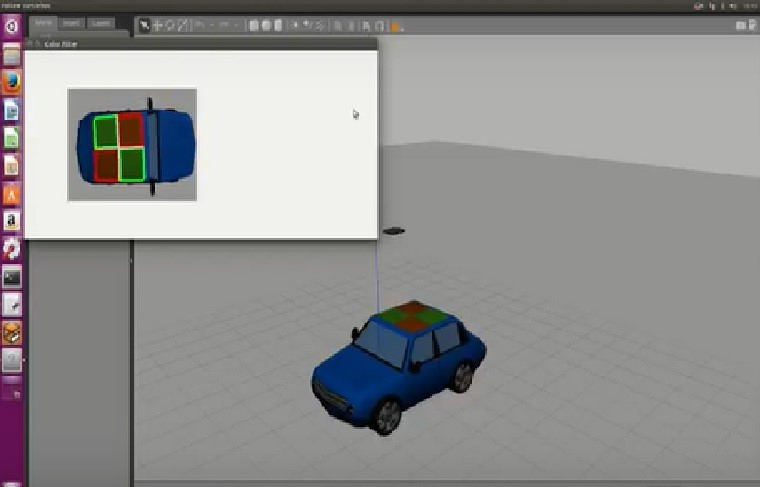
\includegraphics[width=0.4\textwidth]{imgs/TakeOff.jpg}
        \caption{Despegue sobre la baliza del coche.}
	\label{fig:Despegue sobre la baliza del coche}
\end{figure}


\hspace{1cm} Para la realizaci\'on de este experimento con un drone real se sit\'ua la baliza real sobre el suelo y el drone sobre \'esta, y as\'i al despegar ten\'ia un punto sobre el que centrarse. La raz\'on de programar un despegue controlado en vez de en lazo abierto se debe a que el drone real ten\'ia una deriva que le llevaba a desplazarse hacia atr\'as cuando ten\'ia que estar en el sitio. El drone siempre despegaba en esta direcci\'on y hay alrededor de dos segundos en los que no se pueden controlar sus movimientos, por tanto hab\'ia que contar con este desplazamiento. 

\begin{figure}[H]
 \centering
  \subfloat[Despegue vista baliza]{
   \label{f:Vista baliza}
    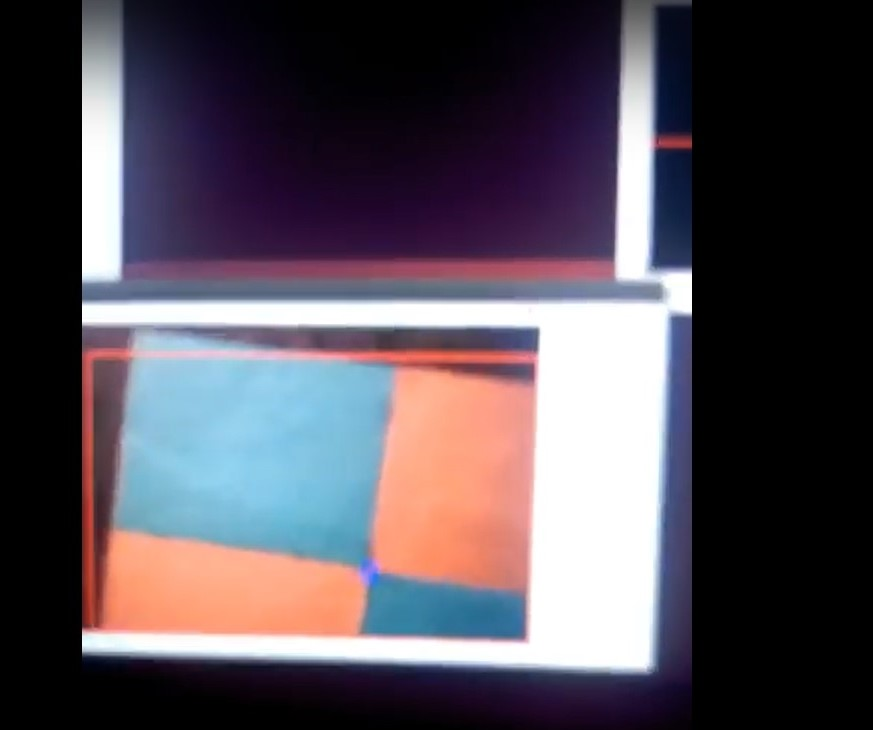
\includegraphics[width=0.4\textwidth]{imgs/takeoff_baliza.jpg}}
  \subfloat[Despegue vista drone]{
   \label{f:Drone}
    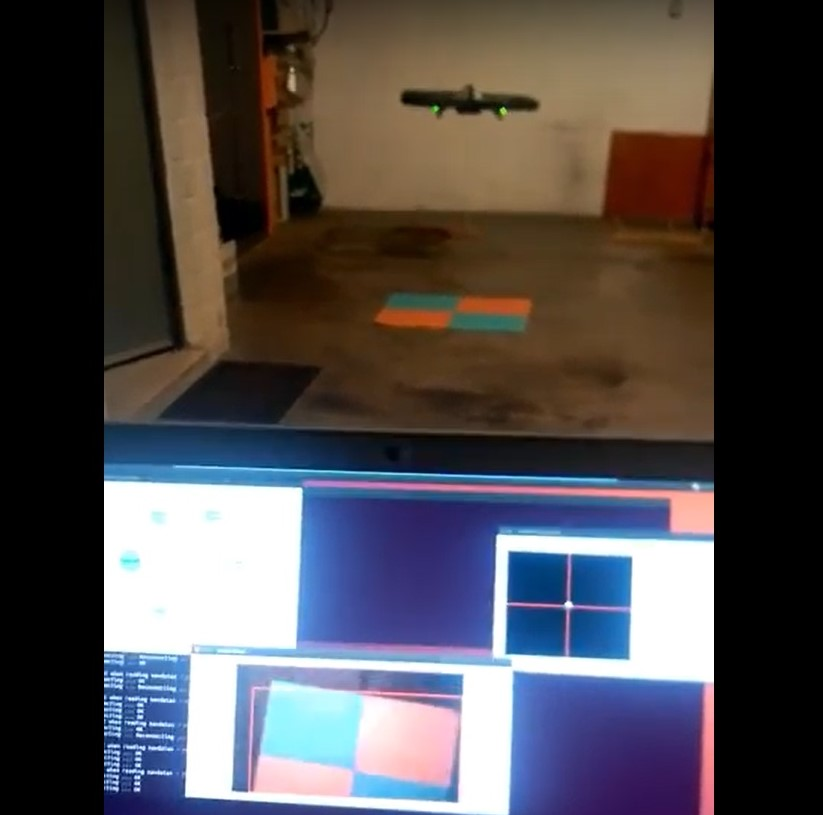
\includegraphics[width=0.4\textwidth]{imgs/takeoff_baliza2.jpg}}
 \caption{Despegue}
 \label{f:Test Despegue}
\end{figure}

Para la realizaci\'on del algoritmo, La duraci\'on del periodo de despegue se controla por tiempo, se ajust\'o en 10 segundos. 
El video de un experimento ilustrativo del despegue del drone real esta disponible en internet. En \'el se puede apreciar un despegue con deriva y la correcci\'on satisfactoria por el software de control desarrollado, de modo que la b\'usqueda de la baliza de destino se inicia mas o menos centrado sobre la baliza de despegue. 
%En el siguiente enlace est\'a el video con el despegue real del drone:\\
\footnote{\url{https://www.youtube.com/watch?v=HVGSlbA1tq4}}

\section{Experimentos de b\'usqueda }
%\hspace{1cm} Para la realizaci\'on de \'esta parte del algoritmo, el drone va movi\'endose en espiral hasta encontrar la baliza, para ya centrarse sobre \'esta. Al principio de los experimentos, el drone se situaba cerca de la baliza para empezar su desplazamiento y que al encontrar la baliza se centrara. Una vez esto funcionaba, se situaba el drone m\'as lejos de \'esta para que en la primera vuelta de la espiral no encontrara ning\'un objeto de inter\'es, pero ya en la segunda vuelta pudiera verlo y se centrara, comprobando de esta forma que las espirales se realizaban de forma correcta. En los primeros experimentos el control, pues solo ten\'ia componente proporcional y el momento que pasaba de no detectar nada a encontrar una posible baliza los movimientos eran muy bruscos, arreglando esto con el control PID. 

\hspace{1cm} Para la realizaci\'on de esta parte del algoritmo, el drone va movi\'endose en espiral hasta encontrar la baliza, para ya centrarse sobre \'esta. Se han realizado diversos experimentos. Por una parte escenarios donde el punto de despegue y el de aterrizaje se sit\'uan muy cerca, por tanto tiene que despegar, detectar la otra baliza y centrarse sobre esta. Por otro lado, escenarios situando lejos la baliza de despegue y de aterrizaje, observando as\'i que el drone ampliaba su recorrido en cada vuelta de espiral que daba. Adem\'as, en ambas pruebas se han controlado las velocidades del drone para evitar movimientos bruscos. 


\begin{figure}[H]
 \centering
    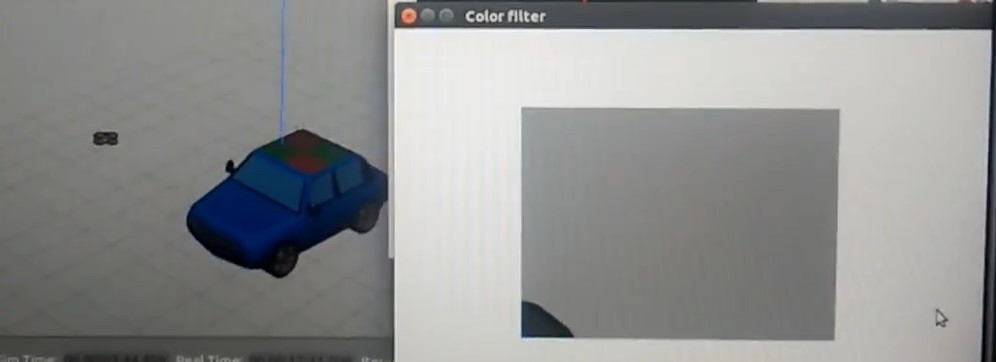
\includegraphics[width=0.33\textwidth]{imgs/busqueda1.jpg}
    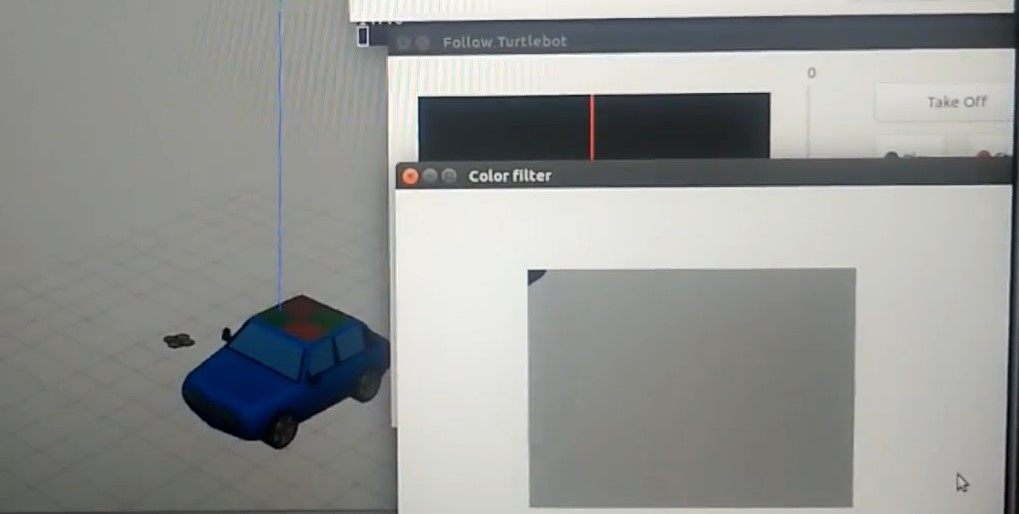
\includegraphics[width=0.32\textwidth]{imgs/busqueda3.jpg}
    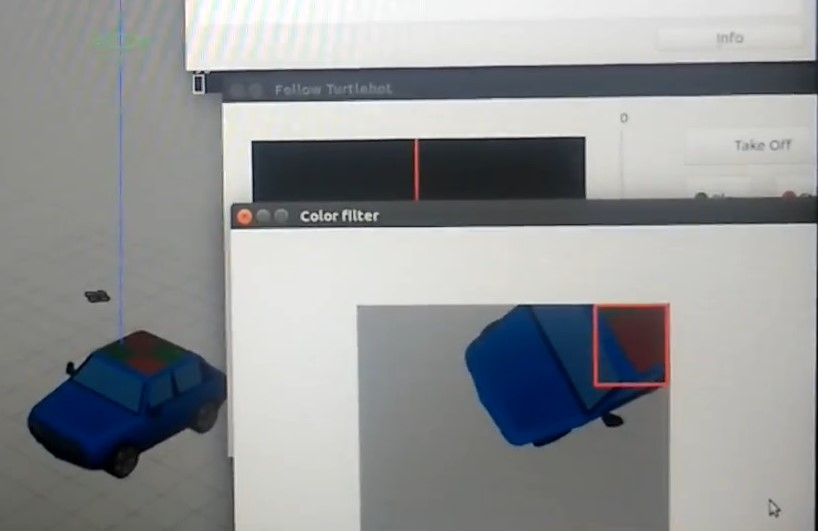
\includegraphics[width=0.29\textwidth]{imgs/busqueda5.jpg}\\
    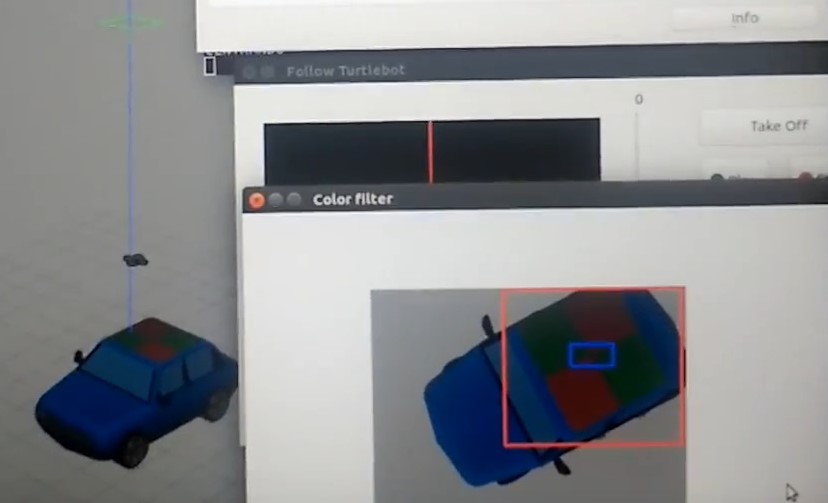
\includegraphics[width=0.39\textwidth]{imgs/busqueda6.jpg}
    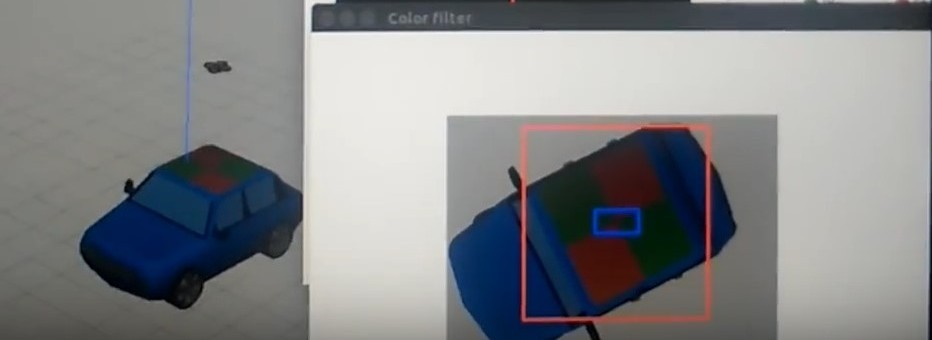
\includegraphics[width=0.4\textwidth]{imgs/busqueda7.jpg}
 \caption{B\'usqueda en espiral en escenario simulado}
 \label{f:Busqueda sobre el simulador}
\end{figure}


%\hspace{1cm} Para las pruebas con del drone real, primero se prob\'o solo que el algoritmo de b\'usqueda era correcto, y que el drone realizaba espirales de forma correcta. Pero despu\'es, al realizar las pruebas finales en espacios m\'as pequeños se modific\'o el algoritmo de b\'usqueda, haciendo que el drone se moviera haciendo cuadrados para tener un mayor control sobre \'este. 

\hspace{1cm} Para las pruebas del drone real, se han realizado tambi\'en dos pruebas principales. Por un lado se han realizado varios tests detectando que el drone hac\'ia espirales de forma correcta, ampliando la trayectoria de forma continua. Por otro lado que al detectar la baliza no realizara movimientos bruscos para centrarse sobre esta. Destacar que para la realizaci\'on de pruebas en lugares poco espaciosos se program\'o otra variante del algoritmo de b\'usqueda, pasando de hacer espirales a hacer cuadrados, para tener un movimiento m\'as controlado del drone. 


\begin{figure}[H]
 \centering
    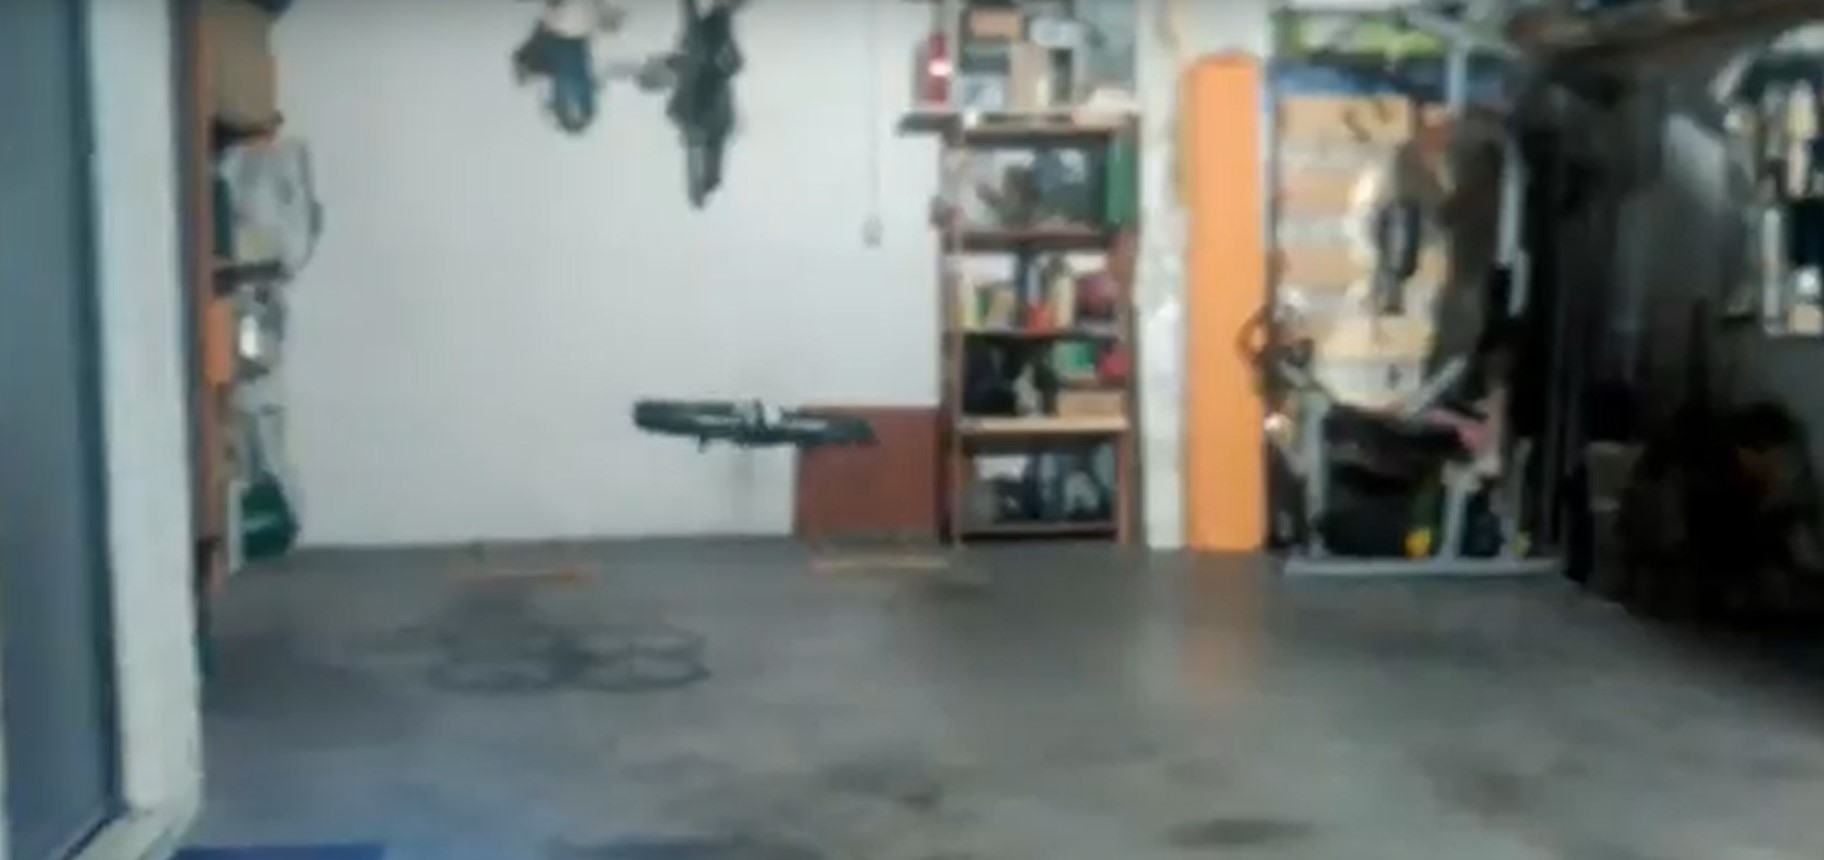
\includegraphics[width=0.33\textwidth]{imgs/busqueda_real1.jpg}
    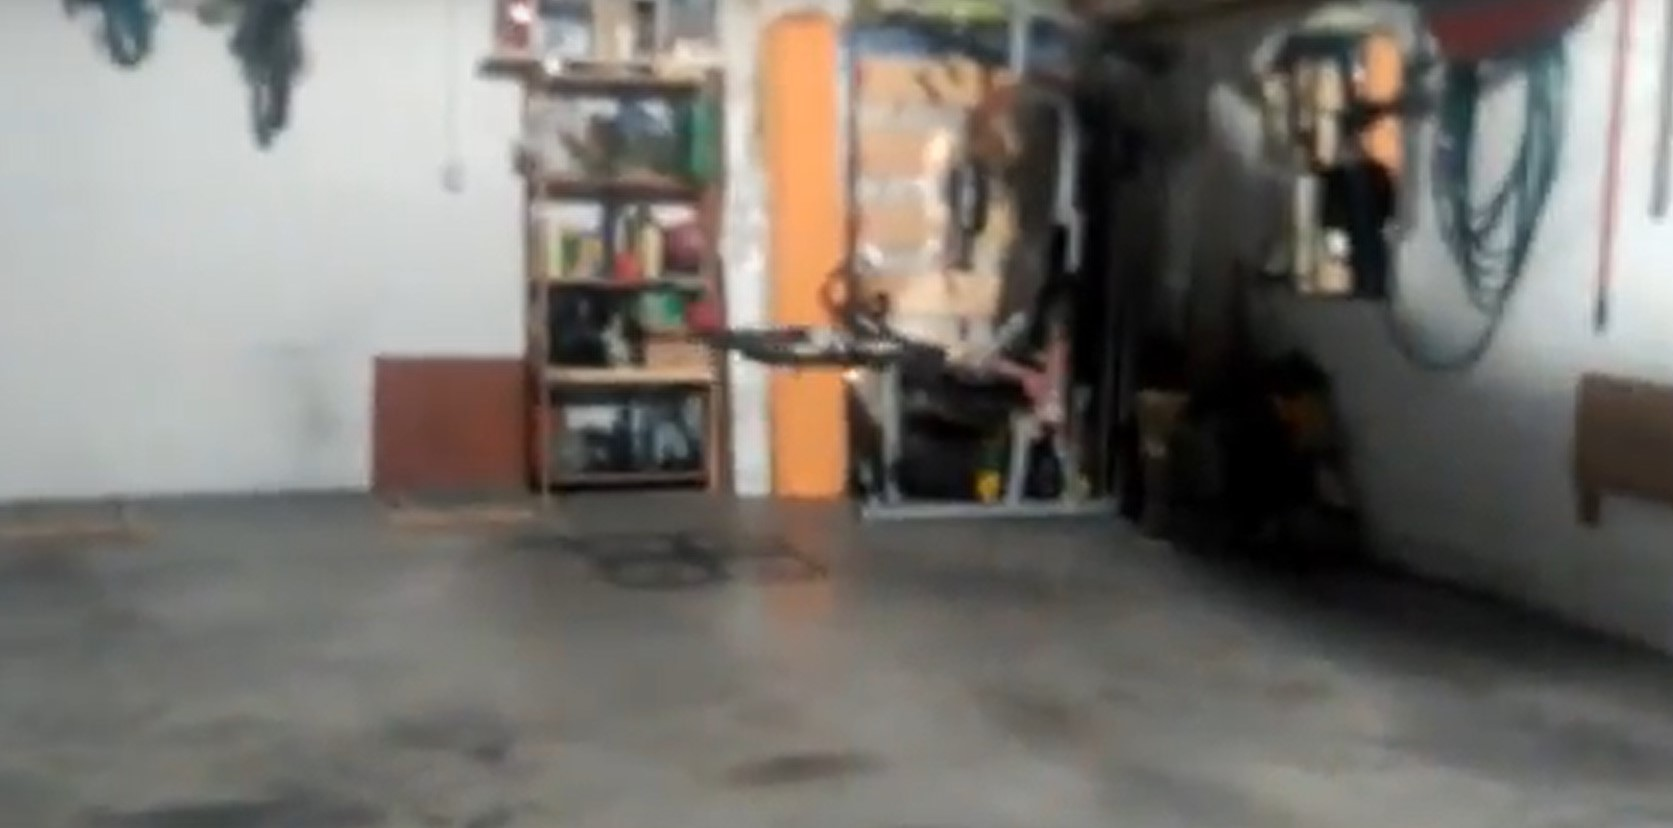
\includegraphics[width=0.32\textwidth]{imgs/busqueda_real3.jpg}
    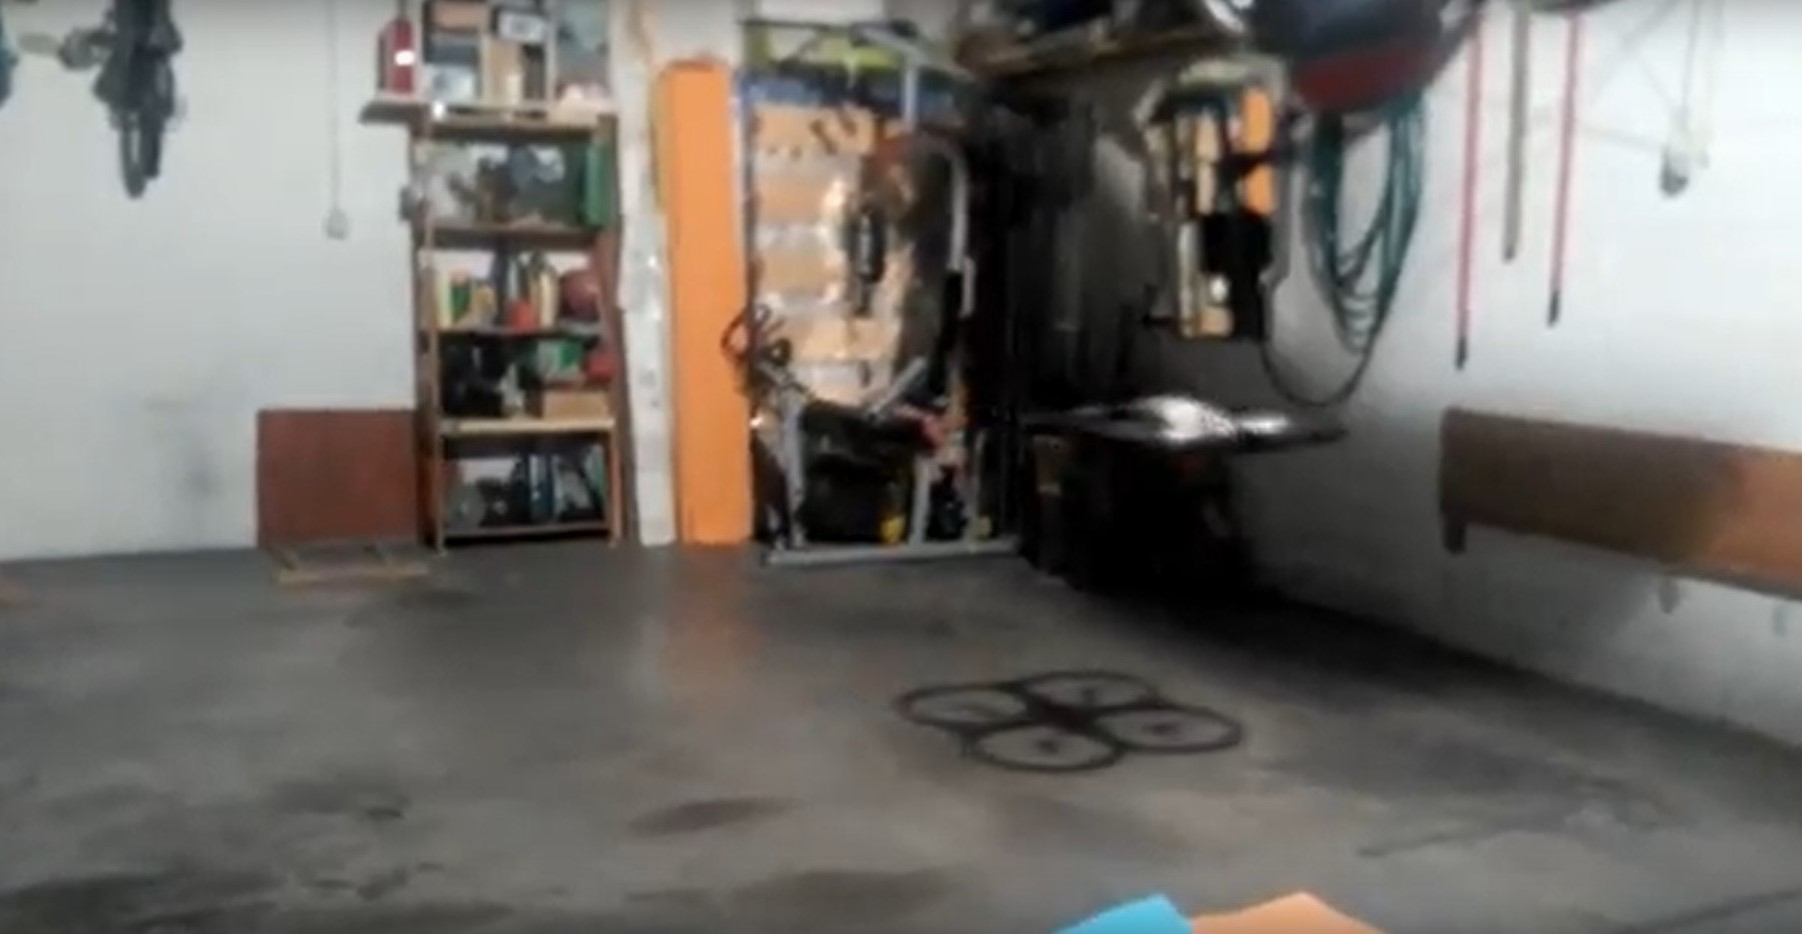
\includegraphics[width=0.30\textwidth]{imgs/busqueda_real5.jpg}\\
    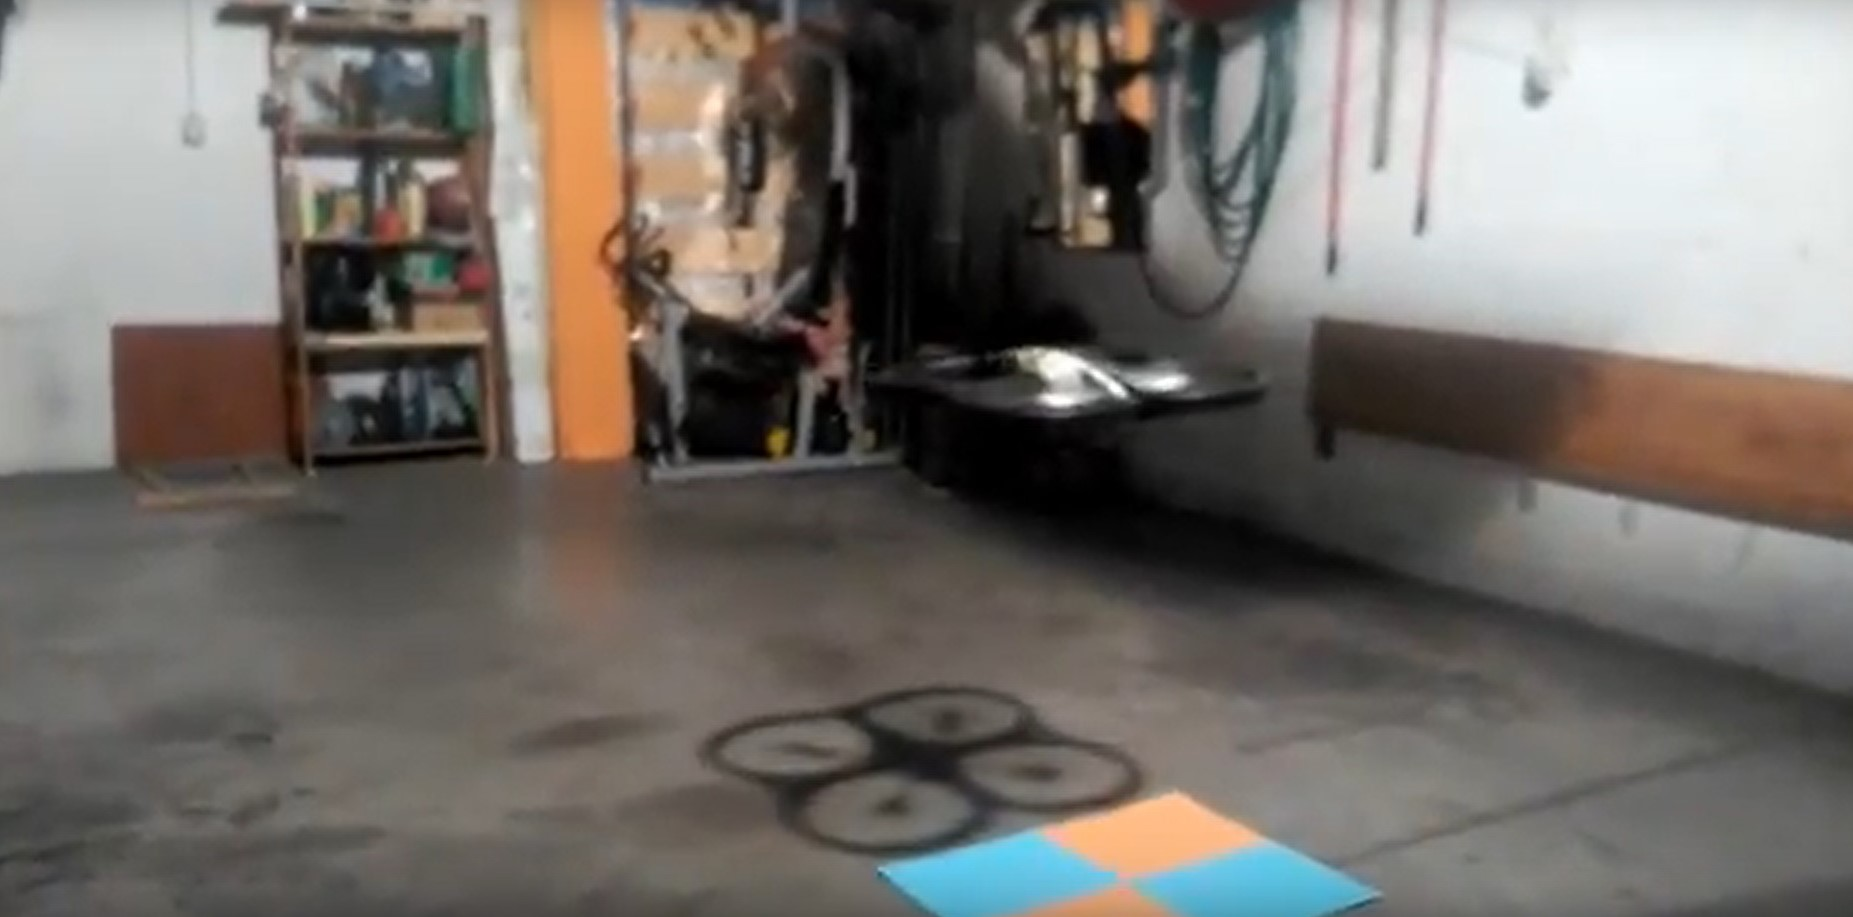
\includegraphics[width=0.4\textwidth]{imgs/busqueda_real6.jpg}
    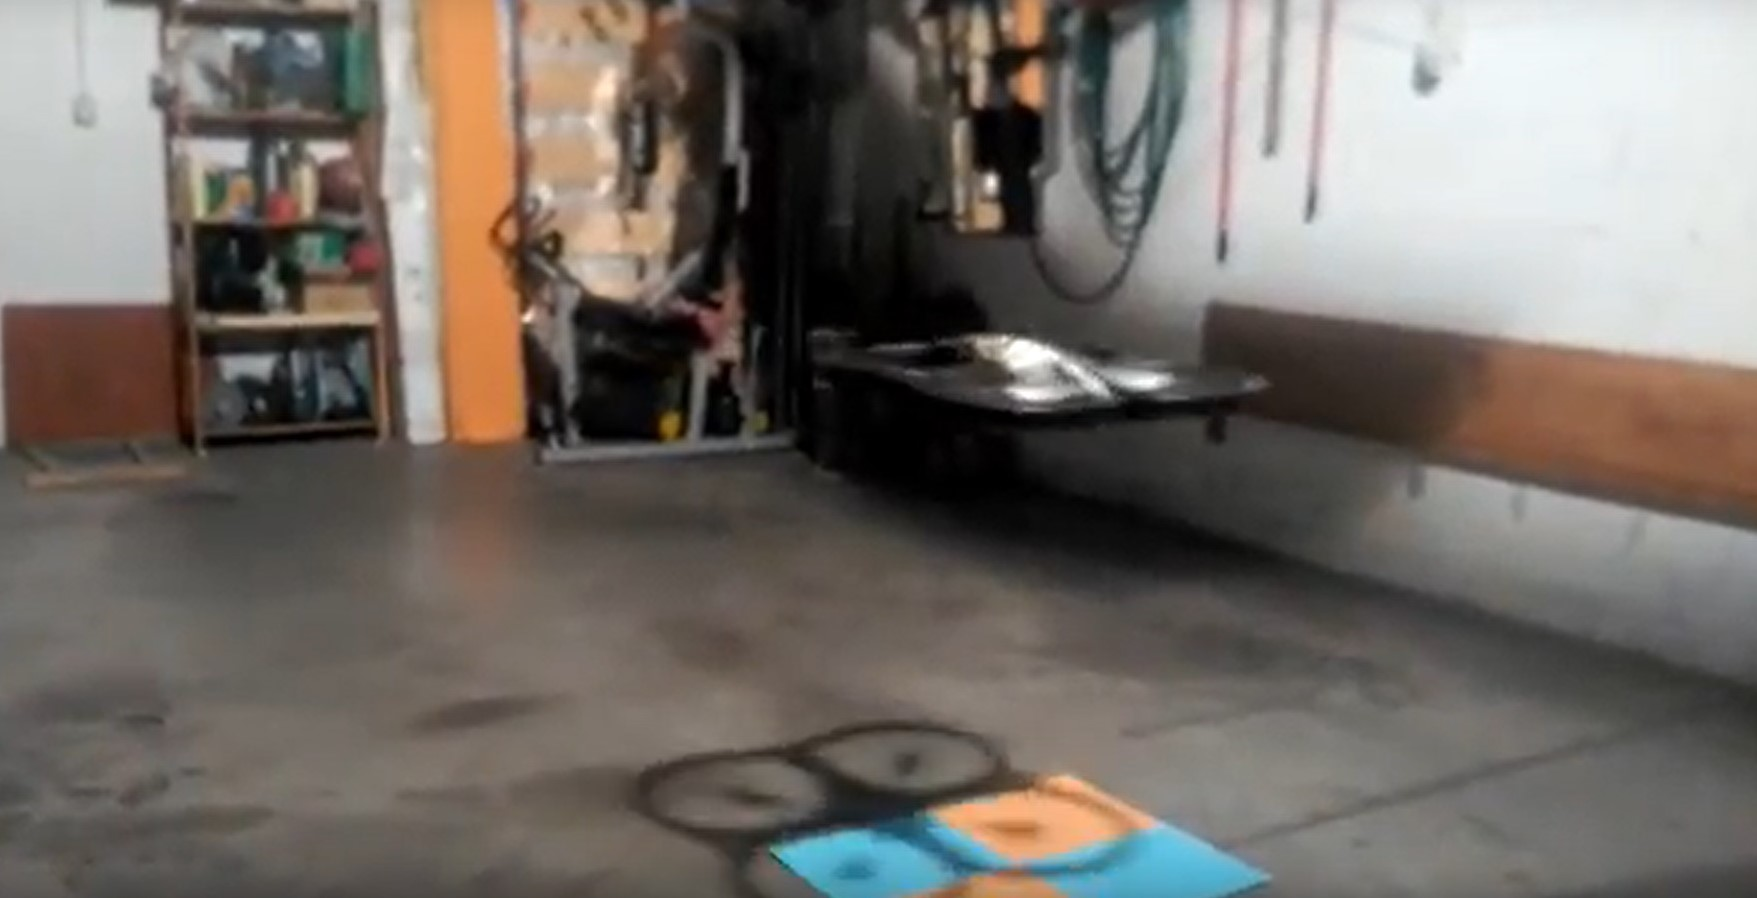
\includegraphics[width=0.38\textwidth]{imgs/busqueda_real7.jpg}
 \caption{B\'usqueda en el escenario real}
 \label{f:Busqueda con el drone real}
\end{figure}


\section{Experimentos de aterrizaje}

\hspace{1cm} En los experimentos de esta parte, se trat\'o de verificar que el drone se centrara sobre la baliza sin realizar movimientos bruscos, una vez que el drone detectaba que estaba pr\'acticamente centrado sobre la baliza, comenzaba a descender, y una vez detectaba que estaba lo suficientemente cerca enviaba la orden de parar.% En estos experimentos la parte de percepci\'on se basan en controlar el centro de la baliza y el \'area, para tener una aproximaci\'on de la distancia que hay a \'esta. 

\begin{figure}[H]
 \centering
    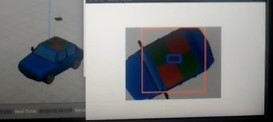
\includegraphics[width=0.45\textwidth]{imgs/landing1_1.jpg}
    \includegraphics[width=0.45\textwidth]{imgs/landing2_1.jpg}
    \includegraphics[width=0.45\textwidth]{imgs/landing3_1.jpg}
    \includegraphics[width=0.45\textwidth]{imgs/landing4_1.jpg}
 \caption{Aterrizaje}
 \label{f:Aterrizaje sobre el simulador}
\end{figure}


\hspace{1cm} En la primera prueba, cuando el drone estaba en el aire se pon\'ia delante de la baliza de un color y al detectarla apagaba motores directamente. En la segunda prueba, cuando el drone estaba en el aire, en lugar de mostrar la baliza a la c\'amara frontal se le mostro a la c\'amara de abajo, probando as\'i el funcionamiento de la camara y que detectaba la baliza que se iba a utilizar. En la tercera prueba, mientras realizaba el algoritmo de b\'usqueda, una vez detectara la baliza aterrizara. En esta prueba los resultados eran buenos, ya que se consegu\'ia que aterrizara, pero por la velocidad que ten\'ia el drone y debido a la inercia, no aterrizaba en el sitio exacto sino que segu\'ia en la misma direcci\'on que ten\'ia anteriormente hasta que se posaba en el suelo y ya se deten\'ia, por lo tanto aterrizaba en las proximidades, pero relativamente tras esto y al añadir el control para centrarse sobre \'esta, se solucion\'o el problema y se consigui\'o que el drone aterrizara verticalmente sobre la baliza. 

\begin{figure}[H]
 \centering
    \includegraphics[width=0.30\textwidth]{imgs/aterrizaje_real1.jpg}
    \includegraphics[width=0.30\textwidth]{imgs/aterrizaje_real2.jpg}
    \includegraphics[width=0.30\textwidth]{imgs/aterrizaje_real3.jpg}\\
    \includegraphics[width=0.30\textwidth]{imgs/aterrizaje_real4.jpg}
    \includegraphics[width=0.30\textwidth]{imgs/aterrizaje_real5.jpg}
    \includegraphics[width=0.30\textwidth]{imgs/aterrizaje_real6.jpg}
 \caption{Aterrizaje}
 \label{f:Aterrizaje con el drone real.}
\end{figure}


\section{Ejecuci\'on t\'ipica del algoritmo completo}\label{sec.algoritmocompleto}
\hspace{1cm} Una vez validada cada una de las partes del algoritmo, tanto perceptivas como de control, se realizaron varios experimentos con todo el sistema integrado.

\hspace{1cm} Este experimento se realiz\'o para comprobar que todo lo que se hab\'ia programado por partes funcionaba tambi\'en si se probaba el algoritmo completo. Las pruebas salieron correctamente.

\hspace{1cm} Sobre el simulador se prob\'o a poner el drone sobre la baliza, que despegaba y se situaba en el centro de \'esta. Una vez pasaron 10 segundos y el drone continuaba en el centro, se hizo que \'este se alejara y perdiera la referencia de la baliza, y comenzara su algoritmo de b\'usqueda. Una vez realizaba las espirales, en el momento que detectaba los colores de la baliza de destino se centraba sobre estos, y una vez estaba aproximadamente centrado, comenzaba a descender hasta que detectaba que estaba a una altura suficiente y se le pod\'ia mandar la orden de aterrizar, pos\'andose as\'i sobre la baliza. 

En la figura \ref{f:Algoritmo completo sobre el simulador} se muestra la secuencia de im\'agenes con el despegue y el drone alej\'andose de la baliza. Las im\'agenes de la b\'usqueda y el aterrizaje est\'an en las figuras \ref{f:Busqueda sobre el simulador} y \ref{f:Aterrizaje sobre el simulador}. La referencia para con el v\'ideo es la siguiente:\\
\footnote{\url{https://www.youtube.com/watch?v=g9ZGJhRWTiY}}

\begin{figure}[H]
 \centering
  \subfloat[Despegue]{
   \label{f:Despegue}
    \includegraphics[width=0.25\textwidth]{imgs/total1.jpg}}
  \subfloat[Despegue]{
   \label{f:Despegue}
    \includegraphics[width=0.25\textwidth]{imgs/total2.jpg}}
	\subfloat[Despegue]{
   \label{f:Despegue}
    \includegraphics[width=0.25\textwidth]{imgs/total3.jpg}}
	\subfloat[Despegue]{
   \label{f:Despegue}
    \includegraphics[width=0.25\textwidth]{imgs/total4.jpg}}\\
	\subfloat[Alejandose de la baliza]{
   \label{f:Alejandose de la baliza}
    \includegraphics[width=0.25\textwidth]{imgs/total5.jpg}}
	%\subfloat[Busqueda]{
  % \label{f:Busqueda}
  %  \includegraphics[width=0.25\textwidth]{imgs/busqueda2.jpg}}
	%\subfloat[Busqueda]{
  % \label{f:Busqueda}
  %  \includegraphics[width=0.25\textwidth]{imgs/busqueda4.jpg}}
	%\subfloat[Busqueda]{
  % \label{f:Busqueda}
  %  \includegraphics[width=0.25\textwidth]{imgs/busqueda6.jpg}} \\
	%	  \subfloat[Aterrizaje]{
  % \label{f:Aterrizaje}
  %  \includegraphics[width=0.25\textwidth]{imgs/landing1.jpg}}
  %\subfloat[Aterrizaje]{
  % \label{f:Aterrizaje}
  %  \includegraphics[width=0.30\textwidth]{imgs/landing2.jpg}}
	%\subfloat[Aterrizaje]{
  % \label{f:Aterrizaje}
  %  \includegraphics[width=0.25\textwidth]{imgs/landing3.jpg}}
	%\subfloat[Aterrizaje]{
  % \label{f:Aterrizaje}
  %  \includegraphics[width=0.25\textwidth]{imgs/landing4.jpg}}
 \caption{Algoritmo completo de navegaci\'on en escenario simulado. }
 \label{f:Algoritmo completo sobre el simulador}
\end{figure}


\hspace{1cm} Para las prueba con el drone real se colocaron dos puntos de referencia. Una baliza sobre la que situarse al despegar. De esta forma al comenzar el algoritmo, cuando detectaba esta baliza se centraba sobre \'esta, y una vez pasaron 10 segundos comenzaba el algoritmo de b\'usqueda. En este punto, el drone se mueve en forma de espiral. En las siguientes im\'agenes puede verse c\'omo en una primera vuelta de la espiral el drone no llega a ver la baliza de destino. Sin embargo, en la segunda vuelta de la espiral ya pasa sobre la baliza, detect\'andola y aterrizando sobre ella. La referencia con el v\'ideo es \footnote{\url{https://www.youtube.com/watch?v=SkpuqEkoryY}}



\begin{figure}[H]
 \centering
  \subfloat[Despegue]{
   \label{f:Despegue}
    \includegraphics[width=0.33\textwidth]{imgs/complete1.png}}
  \subfloat[Despegue]{
   \label{f:Despegue}
    \includegraphics[width=0.33\textwidth]{imgs/complete2.png}}
  \subfloat[Despegue]{
   \label{f:Despegue}
    \includegraphics[width=0.33\textwidth]{imgs/complete3.png}}\\
  \subfloat[B\'usqueda]{
   \label{f:Busqueda}
    \includegraphics[width=0.33\textwidth]{imgs/complete4.png}}
  \subfloat[B\'usqueda]{
   \label{f:Busqueda}
    \includegraphics[width=0.33\textwidth]{imgs/complete5.png}}
  \subfloat[B\'usqueda]{
   \label{f:Busqueda}
    \includegraphics[width=0.33\textwidth]{imgs/complete6.png}}\\
  \subfloat[B\'usqueda]{
   \label{f:Busqueda}
    \includegraphics[width=0.33\textwidth]{imgs/complete7.png}}
  \subfloat[B\'usqueda]{
   \label{f:Busqueda}
    \includegraphics[width=0.33\textwidth]{imgs/complete8.png}}
  \subfloat[Aterrizaje]{
   \label{f:Aterrizaje}
    \includegraphics[width=0.33\textwidth]{imgs/complete9.png}}\\
  \subfloat[Aterrizaje]{
   \label{f:Aterrizaje}
    \includegraphics[width=0.33\textwidth]{imgs/complete10.png}}
  \subfloat[Aterrizaje]{
   \label{f:Aterrizaje}
    \includegraphics[width=0.33\textwidth]{imgs/complete11.png}}
  \subfloat[Aterrizado]{
   \label{f:Aterrizado}
    \includegraphics[width=0.33\textwidth]{imgs/complete12.png}}
 \caption{Algoritmo completo sobre el drone real. }
 \label{f:Algoritmo completo sobre el drone real. }
\end{figure}









\lhead[]{CAPÍTULO \thechapter. Conclusiones}
\chapter{Conclusi\'ones}\label{cap.conclusiones}

\hspace{1cm} Para finalizar, hay que realizar una evaluaci\'on del trabajo realizado, lo aprendido durante este periodo y los objetivos cumplidos. En un primer aspecto, podemos decir que el trabajo ha sido satisfactorio, se ha conseguido un algoritmo que desarrolle un despegue-b\'usqueda-aterriza como se deseaba en un primer momento, adem\'as que para llegar a ello se han superado distintos retos que han ido surgiendo a lo largo de su desarrollo.

\begin{itemize}
	\item El primera parte era realizar un filtro de color para poder aislar los objetos interesantes del resto. Este objetivo se ha conseguido, trabajando principalmente con la librer\'ia OpenCV. Destacar que en el simulador esto fue mas sencillo debido a la nitidez de los colores y que en el drone real llevo mas trabajo, adem\'as se han tenido que hacer diversas pruebas debido a los distintos lugares donde se probaba el drone y la diferencia de colores que hab\'ia debido a la luminosidad, pero al final se consigui\'o un buen filtro, que con ayuda de los operadores morfol\'ogicos (erosi\'on, dilataci\'on, cierre y apertura) nos permit\'ian obtener una imagen de fondo negro y los objetos de los colores deseados en primer plano.

	\item La segunda parte trataba de, una vez obten\'iamos los objetos de los colores deseados, ver si estos eran los objetos que quer\'iamos o no. Por una parte, se miraba el \'area que ten\'ian las figuras, y en caso de no llegar a un tamaño predeterminado, estas se descartaban como posibles objetos. Por otro lado, nos apoyamos en la forma de la baliza, pues los 4 cuadrados que la compon\'ian formaban una cruceta en su centro, la cual era la que se trataba de detectar, por lo que no se depend\'ia solo de unos colores determinados, sino tambi\'en de una figura. 
	
	\item Ya por ultimo, hablando de la parte de control del drone, decir que en el drone real ha sido mucho mas costosa de lo esperado, es una parte que sobre el simulador ha funcionado sin problemas cada vez que se añad\'ia algo, pero al querer trabajar sobre el dron real era muy complicado y cualquier cambio de un valor pequeño supon\'ia gran cambio en la realidad. Todo esto tambi\'en ha sido importante para ver la diferenc\'ia que hay cuando tienes solo un control proporcional y despues le añades las componentes integral y derivativa. 
	
\end{itemize}

\hspace{1cm} Las distintas pruebas y los avances que se han ido dando durante el desarrollo, se han ido validando y estan disponibles en la wiki oficial del proyecto:\\
\underline{\url{http://jderobot.org/Jvela-tfg}}

\hspace{1cm} Por otro lado, mirando los proyectos ateriores a este en los que habia trabajado RoboticsLabs URJC con drones, podemos ver que se ha conseguido algo diferente, ya que en este caso hemos conseguido que un drone navege de forma aut\'onoma gui\'andose por las balizas de color, consiguiendo que vaya de un punto a otro. 


\section{Lineas futuras}

\hspace{1cm}Es importante destacar que estos campo de la rob\'otica y la visi\'on se esta produciendo un importante crecimiento, y añadiendo lo aprendido en el trabajo y como se puede trabajar en el creo que ser\'ia interesante continuar la linea de este proyecto para continuar con el desarrollo y aprendizaje de estas t\'ecnicas. Por un lado, ya hab\'iendo trabajado en la autolocalizaci\'on mediante balizas de colores, ser\'ia interesante trabajar en eso mediante otros sensores como puede ser el GPS, ya que es algo que se esta utilizando mucho actualmente y tiene grandes ventajas. Por otro lado, habiendo trabajado con el software de JdeRobot, ser\'ia interesante seguir viendo las opciones que tiene \'este y trabajar en sus herramientas para segu\'ir sacando provecho a los drones que cada vez son mas completos y vienen con mas sensores, por lo tanto tienen un mayor \'area de trabajo. 







\lhead[]{BIBLIOGRAFÍA}
\bibliographystyle{unsrt}
\bibliography{Memoria}
\addcontentsline{toc}{chapter}{Bibliografía}


\end{document}
